\chapter{\label{chap:chap3} Proposta de trabalho}
% Sergio: será que o título não poderia ser "Projeto", ou "Desenvolvimento do projeto" ou "Organização do projeto" ou "Descrição do protocolo e organização do projeto"?

Seguindo a organização arquitetural da Figura \ref{fig:fig1}, a proposta deste trabalho é fazer com que um \textit{fog node} conheça, de forma autônoma, os recursos disponibilizados por seus vizinhos.
Assim, cada \textit{fog node} saberá quais são os \textit{edge devices} disponíveis na rede, portanto,
o nodo que possui o sensor de chuva saberia que existe um outro nodo na rede capaz de medir a temperatura, por exemplo.


Podemos observar na topologia da Figura \ref{fig:fig1}, que os \textit{fog nodes} não possuem uma um nodo central como servidor.
Em razão da topologia distribuída, se for necessário escalarmos a quantidade de nodos na rede, a mesma não deverá sofrer impactos significativos de performance.

Nas seções a seguir abordaremos a arquitetura, módulos e submódulos que compõem o projeto, bem como resultados esperados, validações e cenários de teste. 

\section{Arquitetura}

Esta Seção define a pilha de protocolos a serem utilizados neste projeto, a justificativa pelas suas escolhas, e por fim, o detalhamento do protocolo proposto.
A pilha de protocolos atuará em conjunto com a organização arquitetural previamente definida na Figura \ref{fig:fig1}.

A fim de facilitar a compreensão da arquitetura deste projeto, a Figura \ref{fig:fig2} explicita a pilha de protocolos que o projeto fará uso para implementar as funcionalidades propostas.

\begin{figure}[htb!]
    \centering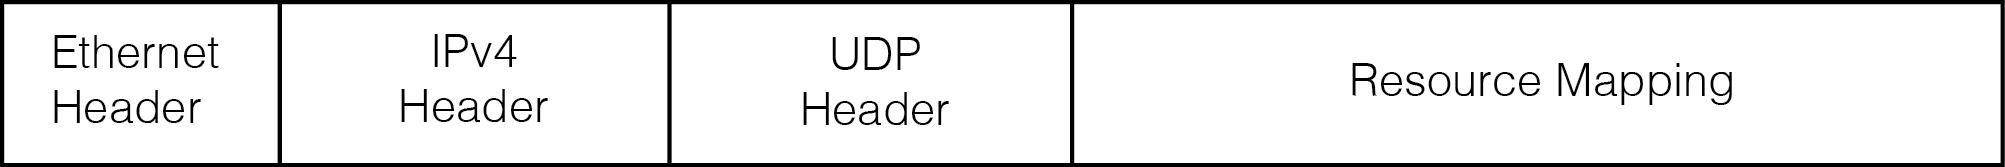
\includegraphics[width=.8\textwidth]{fig2.png}
    \caption%[This figure has a shorter caption now]%
    {\label{fig:fig2} Pilha de protocolos.}
\end{figure}

O modelo de referência TCP/IP é constituido de cinco camadas: física, enlace, rede, transporte e aplicação \cite{tanenbaum2011redes}.
Nesse trabalho, o níveis de rede e transporte (IPv4 e UDP respectivamente) serão utilizados para a implementação do modelo proposto.

A utilização de IPv4 na camada de rede justifica-se pelo fato do protocolo ser empregado em redes locais, que geralmente não necessitam de uma quantidade de endereçamento tão grande 
se comparado ao IPv6, mas não existem impedimentos para que implementações futuras utilizem IPv6 na camada de rede.

Manter o contexto de conexão entre os nodos, utilizando TCP por exemplo, despenderia uma quantidade de trafego desnecessário na rede.
Visto que a simplicidade é um dos objetivos deste trabalho e que transitar uma pequena quantidade de dados a cada requisição aumenta o desempenho da solução,
a utilização de datagramas UDP faz sentido neste protocolo

A Figura \ref{fig:fig12} apresenta, de forma detalhada, a estrutura dos dados contidos no protocolo \textit{Resource Mapping}.

\begin{figure}[htb!]
    \centering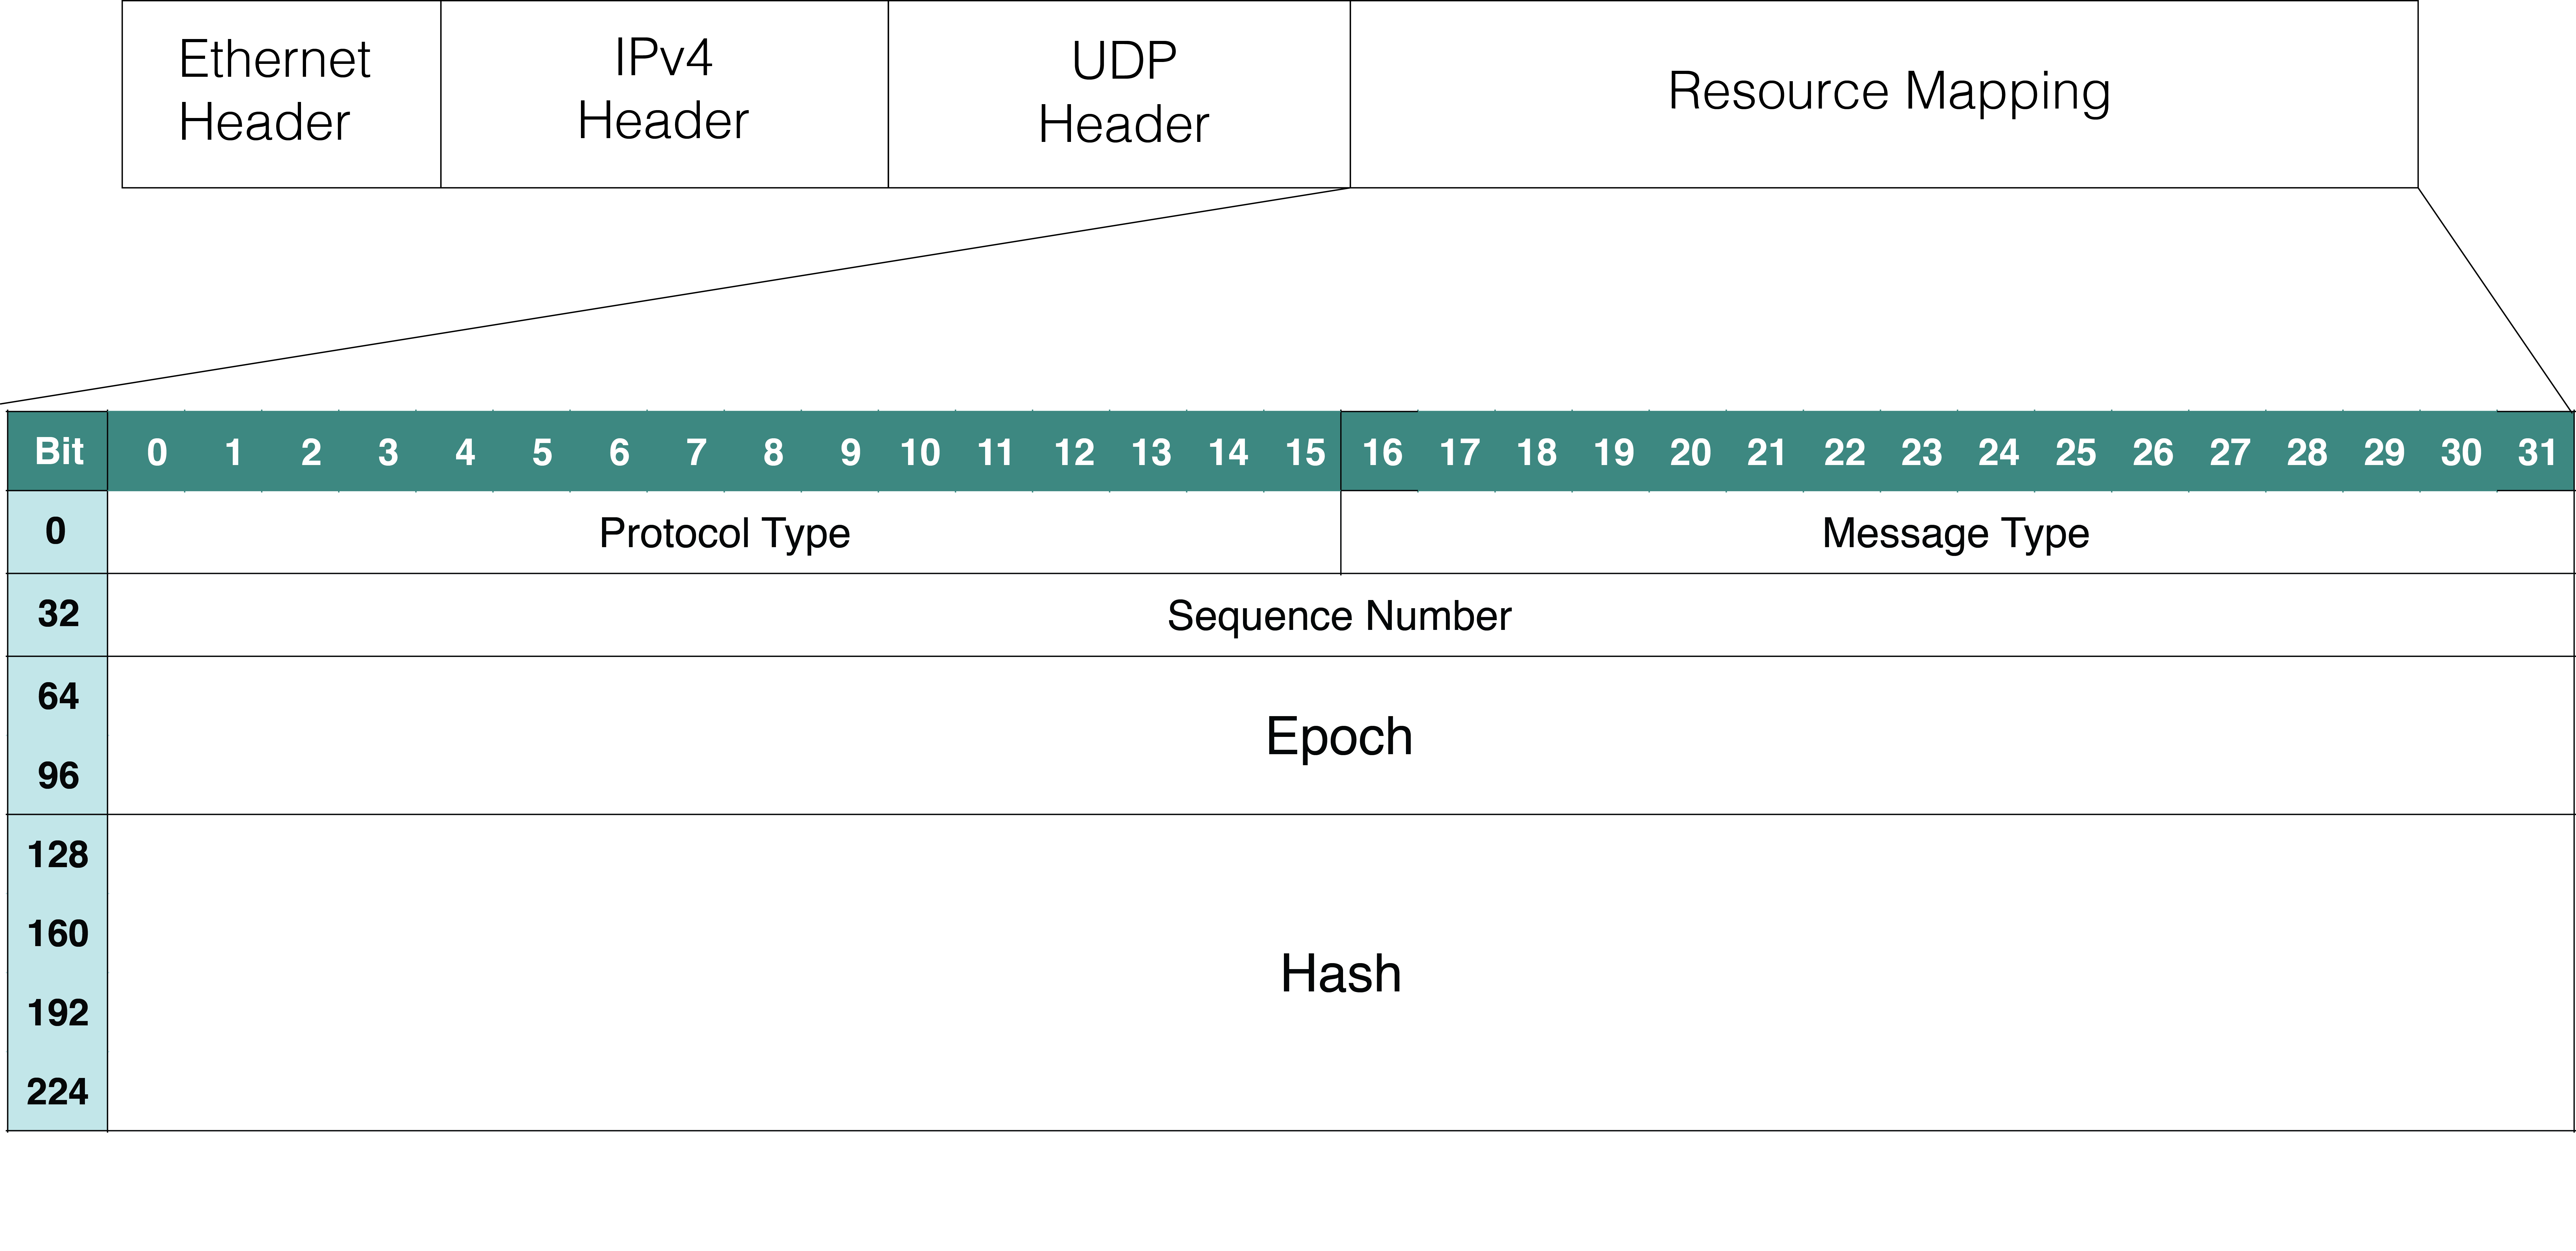
\includegraphics[width=.8\textwidth]{fig12.png}
    \caption%[This figure has a shorter caption now]%
    {\label{fig:fig12} Detalhamento Resource Mapping.}
\end{figure}

\begin{itemize}
\item O campo Protocol Type é reservado para indicar a forma de encapsulamento do pacote.
\item Atualmente existem dois tipos de Messages Types possíveis, keep alive e acknowledgement.
\item Sequence Number tem o intuito de identificar o pacote enviado.
\item O campo Epoch é utilizado para indicar alterações nos recursos providos pelo fog node.
Sendo assim, quando um recurso é adicionado ou removido de um fog node, o campo Epoch é acrescido em uma unidade.
\item O campo Hash utiliza a função de criptografia MD5 para validar a integridade dos demais campos contidos no pacote.
\end{itemize}

O protocolo proposto, intitulado \textit{Resource Mapping}, como apresentado nas Figuras \ref{fig:fig2} e \ref{fig:fig12}, atuará na camada de aplicação do modelo de referência TCP/IP \cite{tanenbaum2011redes} e será responsável por padronizar, descobrir e sincronizar os nodos da névoa.
Os maiores desafios neste modelo proposto são manter o estado global dos recursos acessível a todos os nodos, e garantir que o desempenho seja satisfatório com o objetivo permitir a escalabilidade da solução.


\section{Módulos}

De forma geral, cada nodo da rede deverá manter uma lista com os endereços IP`s que fazem parte do mapeamento.
Atrelado à cada endereço IP, deverá haver uma lista com os recursos providos por este.
Em vista disso, cada nodo portará um mapeamento global de recursos disponíveis na névoa.

O detalhamento das funcionalides que o projeto deverá dispor, tal como ilustrações relacionadas aos fluxos, serão abordadas nas proximas subseções.

\subsection{Gerenciamento de recursos}

Observando a Figura \ref{fig:fig1}, notamos que há comunicação entre um fog node e seus respectivos edge devices.
A comunicação entre estes será executada utilizando o protocolo CoAP, todavia os dados que os edge devices fornecerão aos fog nodes serão tratados de forma simulada.

O gerenciamento de recursos deverá prever alguns casos que, por vezes, possam suceder. Dentre alguns dos eventos possíveis está
o acréscimo ou remoção de um edge device vinculado à algum fog node.
Utilizar CoAP para as funcioalidade de inclusão e exclusão de recursos faz sentido, uma vez que este prevê meios para tal.

Segundo a definição de POST do protocolo CoAP, sua função é determinada pelo servidor que está recebendo a requisição e pelo do recurso referenciado na URI.
Geralmente a sua utilização resulta na criação ou atualização de um recurso\cite{rfc7252}.
Já a mesma RFC define o método DELETE como sendo um método de remoção de recursos baseado em URIs\cite{rfc7252}.
Nessa perspectiva, portanto, o uso do método POST faz sentido para gerarmos \textit{(CoRE) Link Format} e o método DELETE para removermos.


\subsection{Descoberta de recursos}


Partindo do pressuposto que os nodos da névoa já possuem seus recursos devidamente criados e acessíveis via CoAP,
como primeiro passo do mapeamento devemos considerar a entrada de um novo nodo na rede.
No momento em que o nodo dispor de um endereço IP válido, este deverá enviar um pacote para o endereço de multicast indicando que possui recursos a serem disponibilizados.


Ao receberem o pacote enviado por multicast, os nodos que desejarem saber quais recursos estão sendo providos por este novo membro, deverão realizar uma Requisição
unicast para a URI \textit{/.well-known/core} utilizando o protocolo CoAP.
Vale lembrar que este fluxo de requisição e resposta, utilizando a URI \textit{/.well-known/core}, faz com que o nodo requisitado retorne todos seus recursos ao solicitante.

\begin{figure}[H]
    \centering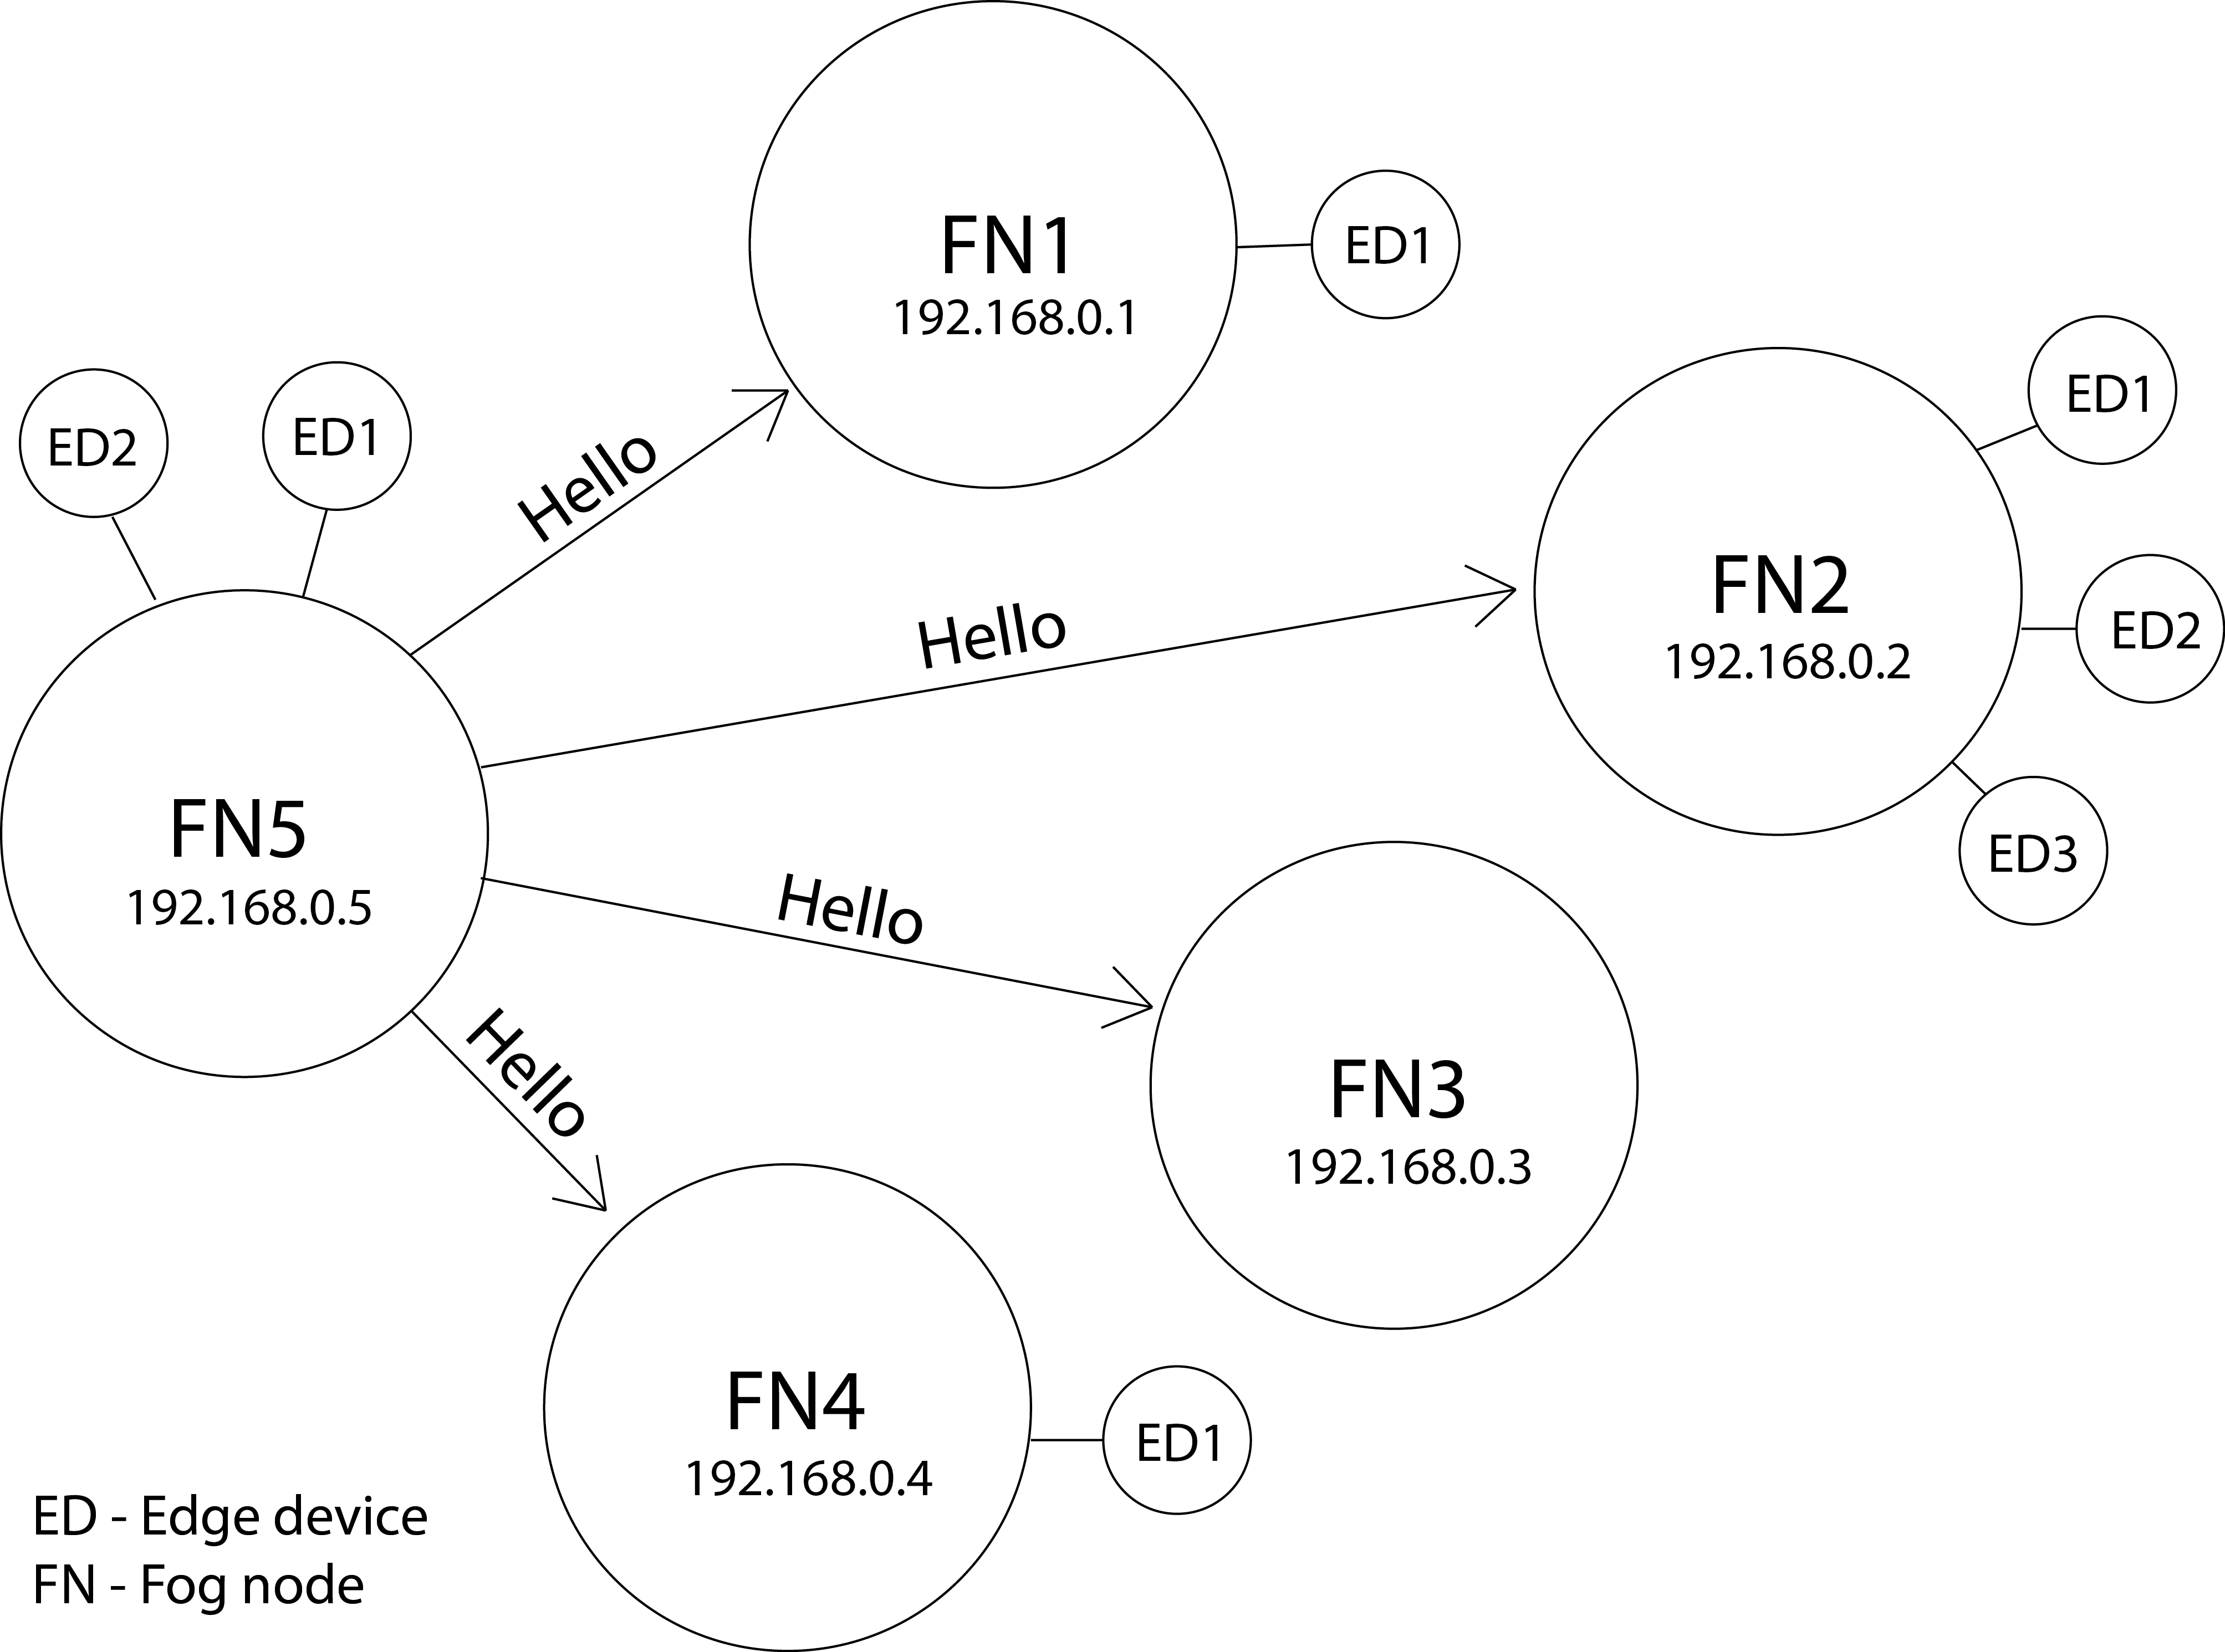
\includegraphics[width=.8\textwidth]{fig5.png}
    \caption%[This figure has a shorter caption now]%
    {\label{fig:fig5} Nodo entrando na névoa.}
\end{figure}

A topologia da névoa utilizada nas Figuras \ref{fig:fig5} e \ref{fig:fig6} é definida por fog nodes enumerados de um a cinco, sendo o nodo FN5 o último a entrar na rede.
A figura \ref{fig:fig5} demonstra o nodo FN5 entrando na névoa e, portanto, deverá anunciar-se por multicast indicando que possui recursos a serem disponibilizados.

Após FN5 enviar mensagem de Olá por multicast, os nodos FN1, FN2 e FN4 realizam a Requisição CoAP diretamente ao FN5 afim de obter os recursos disponíbilizados por ele,
já o nodo FN3, por não estar executando o protocolo de mapeamento, não.

\begin{figure}[H]
    \centering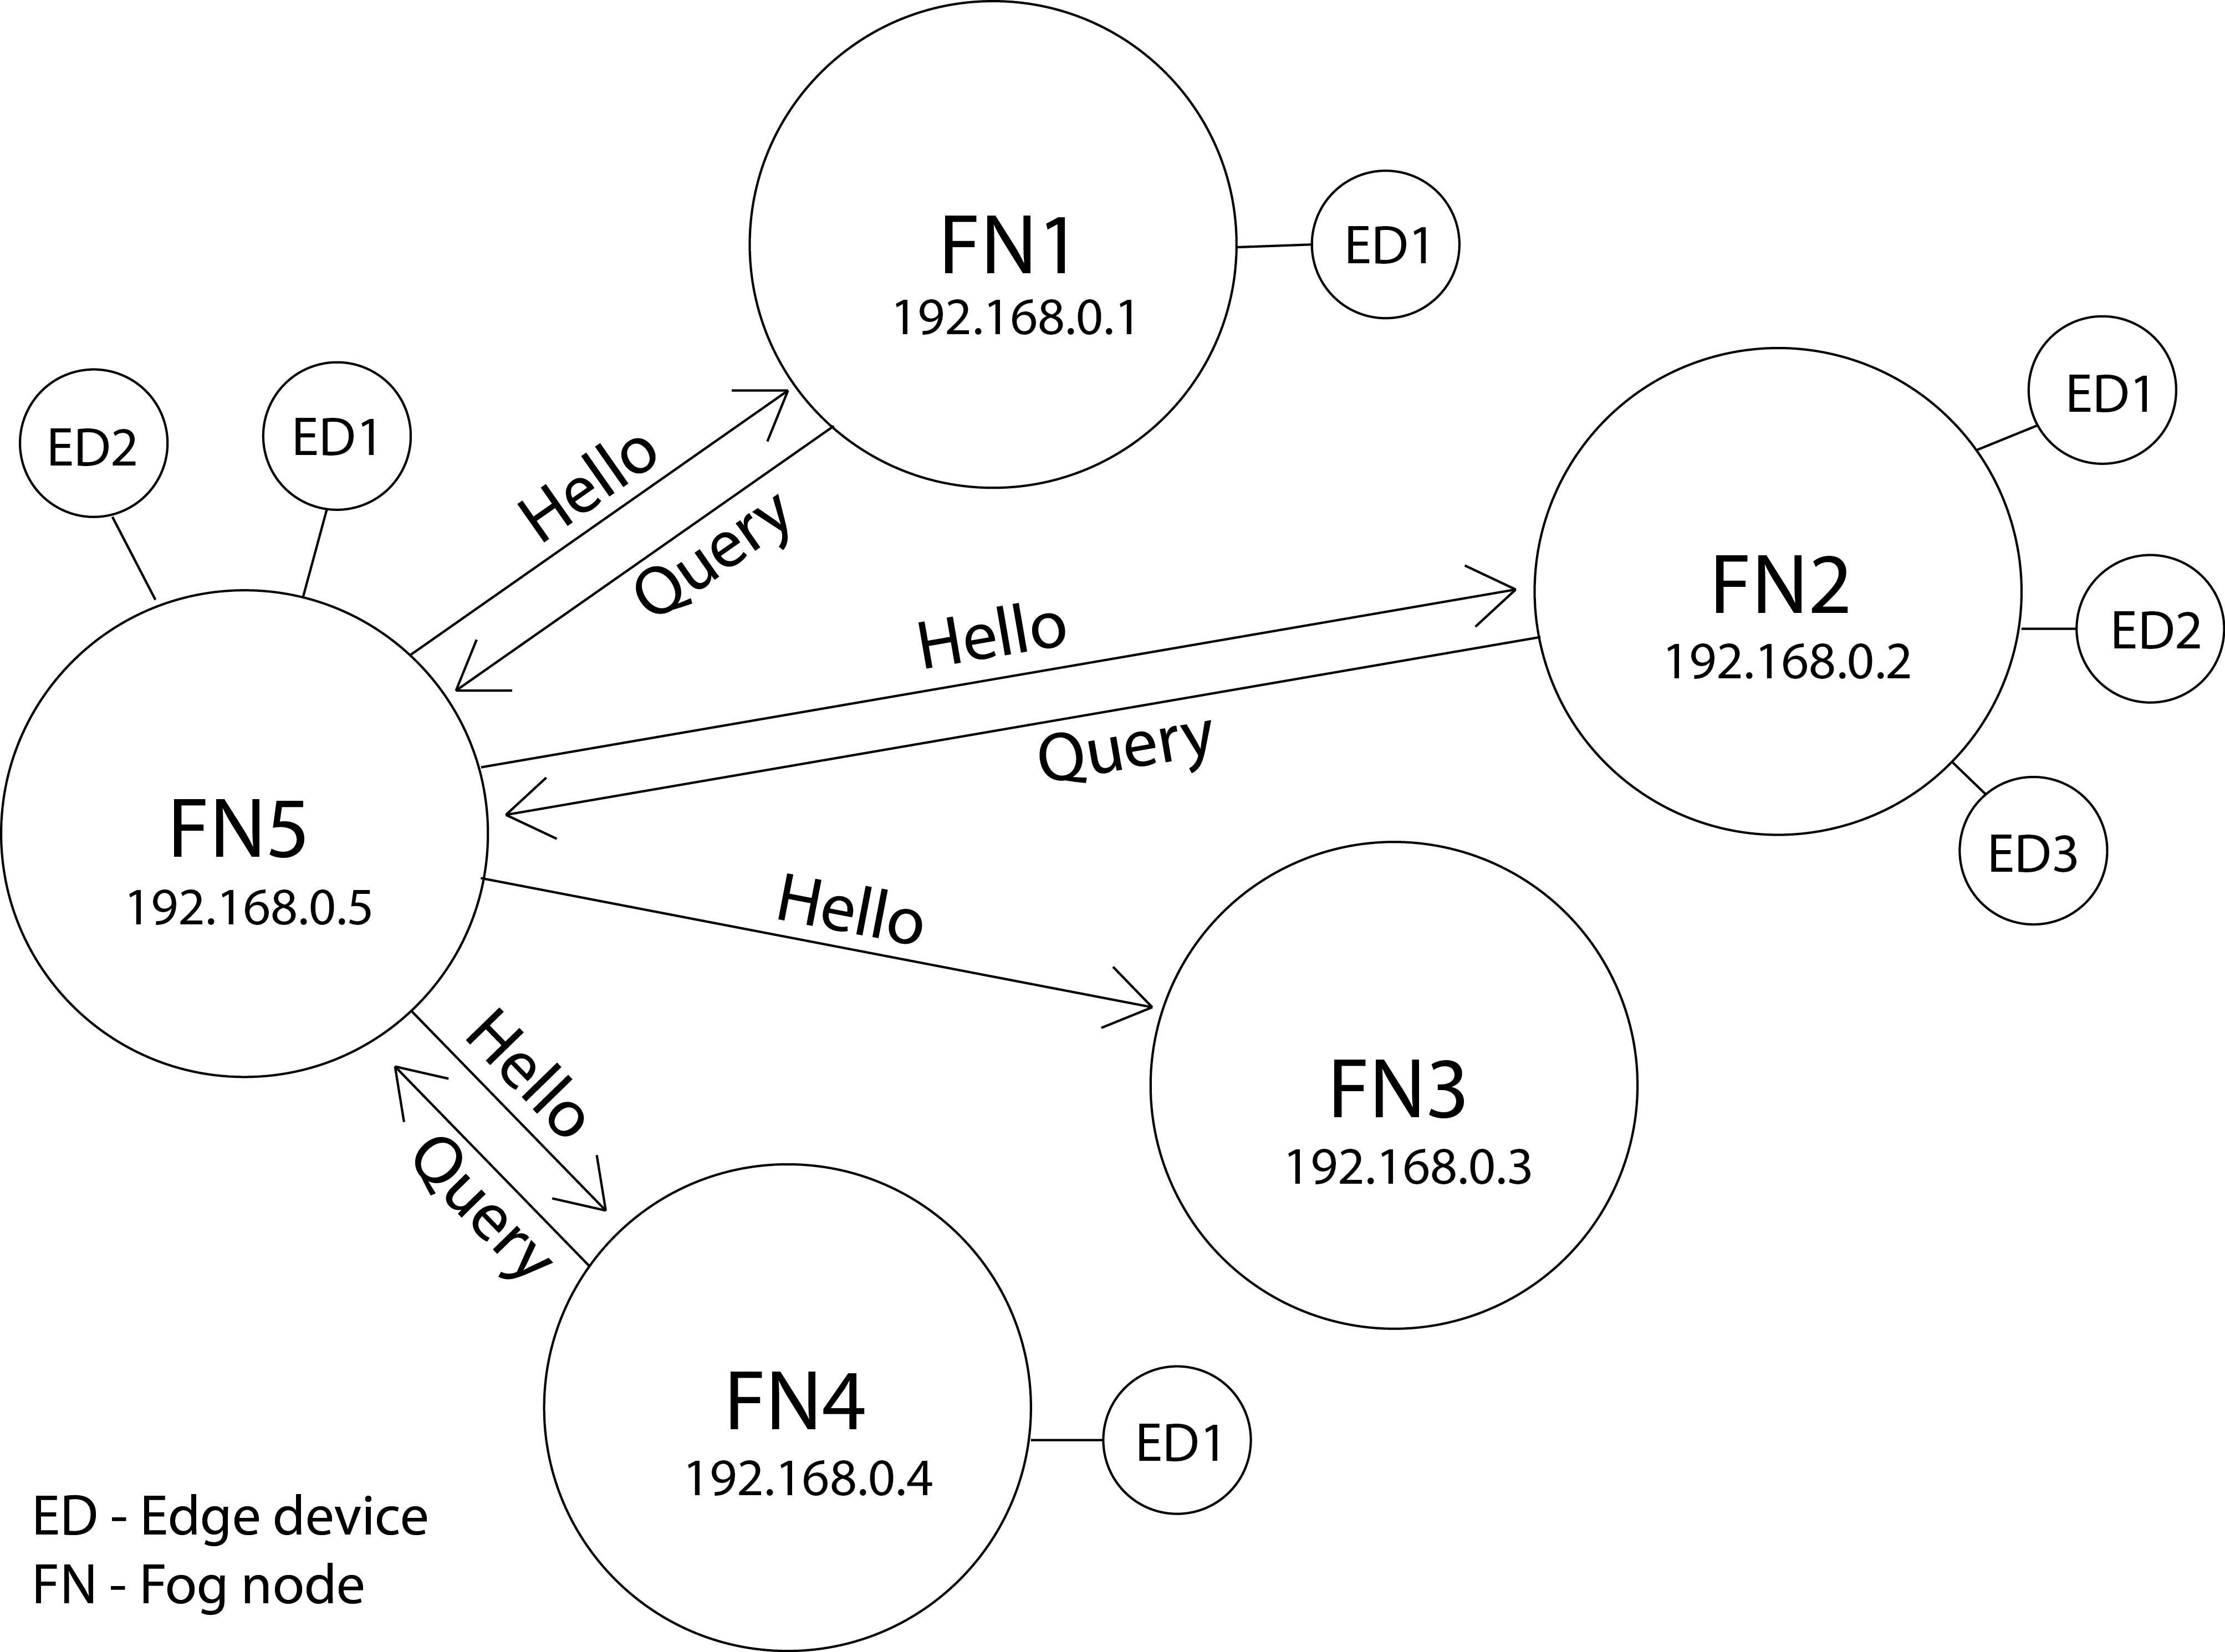
\includegraphics[width=.8\textwidth]{fig6.png}
    \caption%[This figure has a shorter caption now]%
    {\label{fig:fig6} Nodos realizando Requisição.}
\end{figure}


\subsection{Gerenciamento de recursos}

A manutenibilidade da lista de recursos globais é relevante para que a implementação do protocolo tenha sucesso, pois, a névoa deverá saber quando um nodo, ou recurso dele, deixou de fazer parte da rede.
Para tal, faz-se necessário a utilização de alguns mecanismos de controle.
Esses controles são realizados em duas esferas, a primeira trata da inserção ou remoção de um nodo na rede,
já a segunda refere-se a inserção ou remoção de um edge device vinculado a um nodo qualquer.


Inicialmente abordaremos a entrada e saída de nodos da névoa, e para esta subseção será utilizado o cenário da Figura \ref{fig:fig6} quando necessário.
O Pseudocódigo \ref{alg:alg1} demonstra, de forma sucinta, a política de atualização que cada nodo deverá implementar no recebimento de mensagens de keep alive.


\begin{algorithm}[H]
    \begin{center}
        \begin{algorithmic}[1]
            \STATE \textbf{function} $\text{Policy(ip, epoch, myEpoch)}$
            \STATE \hspace{\algorithmicindent} \textbf{if} $\text{exists(ip)}$
            \STATE \hspace{\algorithmicindent} \hspace{\algorithmicindent} \textbf{if} $\text{epochHasChanged(epoch, myEpoch)};$
            \STATE \hspace{\algorithmicindent} \hspace{\algorithmicindent} \hspace{\algorithmicindent} $\text{resources = getResourcesCoAP(ip, '/.well-known/core')};$
            \STATE \hspace{\algorithmicindent} \hspace{\algorithmicindent} \hspace{\algorithmicindent} $\text{update(ip, resources)};$
            \STATE \hspace{\algorithmicindent} \textbf{else}
            \STATE \hspace{\algorithmicindent} \hspace{\algorithmicindent} $\text{resources = getResourcesCoAP(ip, '/.well-known/core')};$
            \STATE \hspace{\algorithmicindent} \hspace{\algorithmicindent} $\text{insert(ip, resources)};$
            \STATE \hspace{\algorithmicindent} $\text{sendAcknowledgement(ip)};$

        \end{algorithmic}
    \end{center}
    \caption[Política de atualização de recursos]%
        {\label{alg:alg1} Política de atualização de recursos.}%
    \end{algorithm}

No momento em que o nodo recebe a resposta da chamada de função \textit{getResourcesCoAP}, contendo os recursos providos pelo nodo requisitado, aquele deverá armazenar as informações em uma estrutura de dados adequada.
Essa estrutura de dados estará implementada em todos os nodos da névoa, e a partir dela será possível realizar o gerenciamento dos recursos de forma simples e eficiente.
O trecho abaixo define, por ora, o formato dos dados que serão utilizados em cada nodo.


\begin{verbatim}
    Fog = {
        string ip;
        string resources[];    
    };
    Fog fogs[];
    string myResources[];
\end{verbatim}

De posse da Figura \ref{fig:fig6} como cenário, do algoritmo de atualização \ref{alg:alg1}, e da estrutura de dados previamente descrita,
demonstramos abaixo o estado em que se encontram os dados armazenados em FN2 após a aplicação do método.

\begin{verbatim}
    fogs: [
        {
            ip: '192.168.0.1',
            resources: [ 'ED1' ]
        },
        {
            ip: '192.168.0.3',
            resources: [ ]
        },
        {
            ip: '192.168.0.4',
            resources: [ 'ED1' ]
        },
        {
            ip: '192.168.0.5',
            resources: [ 'ED1', 'ED2' ]
        }
    ];
    myResources: [ 'ED1', 'ED2', 'ED3' ];
\end{verbatim}

Visto isso, é imprescindível que os nodos mantenham seus dados consistentes, pois, após adicionar o novo nodo em sua lista de fogs, o protocolo precisa ser capaz de perceber quando um elemento
deixou de fazer parte do processo. Assim, a manutenção dos estados será abordado de forma similar as mensagens de \textit{keep alive} utilizadas no protocolo BGP.
Mensagens de keep alive são adotadas para que os nodos da rede avisem seus vizinhos que ainda estão em operação, pois, sem esse procedimento seria difícil
saber quando remover um IP da lista de recursos. Portanto, para manter a lista atualizada, este protocolo implementará mensagens desse tipo.

As mensagens de keep alive serão transmitidas sob multicast em um intervalo de trinta segundos, porém, este é apenas um valor arbitrário, e pode ser alterado
para que a solução obtenha uma melhor eficiência.
Após o recebimento da mensagem de keep alive, os nodos deverão respondê-las indicando que ainda estão em operação.
Caso o nodo não responda a mensagem de keep alive, este será marcado como parcialmente inativo pelo remetente da mensagem.
Quando o nodo solicitante realizar outra mensagem de keep alive e o nodo que já estava marcado com parcialmente inativo não responder, o mesmo será removido da lista de recursos do
solicitante, e assim é possível saber quando um nodo deixou de fazer parte da névoa.
Para realizar este controle será preciso adicionar na estrutura \textit{Fog} a propriedade boleana, denominada \textit{isReplyingKeepAlive}, que indica se o nodo está respondendo a solicitações de keep alive.

As mensagens de keep alive mantém os nodos informados sobre o estado de seus vizinhos, mas não conseguem indicar informações relacionadas aos edge device.
Consequentemente, não é possível saber quando um edge device parou ou iniciou sua operação em um nodo ativo.

Para que seja possível detectarmos esse tipo de comportamento, o protocolo proposto deverá implementar a técnica denominada \textit{época},
e servirá para que os nodos mantenham ciênia sobre o estado dos edge devices de seus vizinhos de rede.
Para isso, uma nova propriedade denominada \textit{epoch}, do tipo inteiro, deverá ser adicionada a estrutura de dados, e estará presente tanto no nodo em si quanto em cada item da lista de fogs.
O valor da \textit{epoch} será incrementado em uma unidadade a toda alteração observada no nodo, seja pelo acréscimo ou pela remoção de edge devices.

Esta observação atuará realizando requisições para a URI /.well-known/core no endereço de loopback do próprio nodo,
assim, obterá seus recursos disponíveis e poderá comparar com os que possui armazenado em sua estrutura de dados.
Havendo divergências, como mencionado anteriormente, a propriedade época será incrementada em uma unidadade.

A partir de agora, então, todas as mensagens de keep alive deverão conter a época do nodo que está realizando o multicast.
Assim, todo nodo que receber a mensagem poderá comparar a época recebida na mensagem com a época que possui armazenada em sua lista de fogs referente ao remetente da mensagen.
Havendo divergência de épocas, este deverá realizar uma nova requisição para atualizar sua lista de recursos referente aquele nodo em específico.

Após as alterações realizadas na estrutura de dados, abaixo temos o novo modelo que suportará as funcionalidades propostas.
\begin{verbatim}
    Fog = {
        string ip;
        string resources[];
        int epoch;
        boolean isReplyingKeepAlive;
    }
    Fog fogs[];
    string myResources[];
    int epoch;
\end{verbatim}


\section{Configuração da névoa}
% Sergio: Essa seção pode fazer parte do capítulo 4, seção "Ambiente de simulação"

Em um primeiro momento a névoa foi construída de forma simulada utilizando a ferramenta Common Open Research Emulator (CORE)\cite{coregui}.
Para os primeiros experimentos a ferramente obteve resultados satisfatórios, porém quando foi necessário escalarmos a solução ela se mostrou ineficiente.
A ineficiência estava na criação dos nodos e na execução dos protocolos CoAP e Resource Mapping, uma vez que eles deveriam ser executados em todos os hosts da rede e não havia 
meios de automatizar este processo.

Esta automatização foi implantada utilizando a SDK de gerenciamento de containers Docker para Python, desta forma, foi possível criarmos névoas com tamanhos arbitrários
e, portanto, a ascalabilidade da solução pode ser amplamente testada\cite{dockersdk:2018}.

Cabe ressaltar que containers Docker\cite{docker:2018} consomem recursos da maquina hospedeira, tais como memória, processamento, disco rígido.
Portanto, a criacao de containers da névoa fica atrelado a quantidade de recursos que esse host pode proporcionar.

Cada container executa uma distrbuição Linux chamada Alpine, de aproximadamente 5Mb, que possui apenas as funcioalidades básicas de um sistema operacional\cite{linuxalpine:2018}.
O fato da distribuição ser Open Source faz com que existam customizações da mesma, e neste projeto foi utilizado a customização que inclui a versão 2.7 da linguagem Python.
Tal customização faz-se necessária para a execução dos protocolos CoAP e Resource Mapping.


A Figura \ref{fig:fig13} não só expõe os elementos que fazem parte da arquitetura de cada container, mas também os detalha em nível de requisições entre sí.


\begin{figure}[H]
    \centering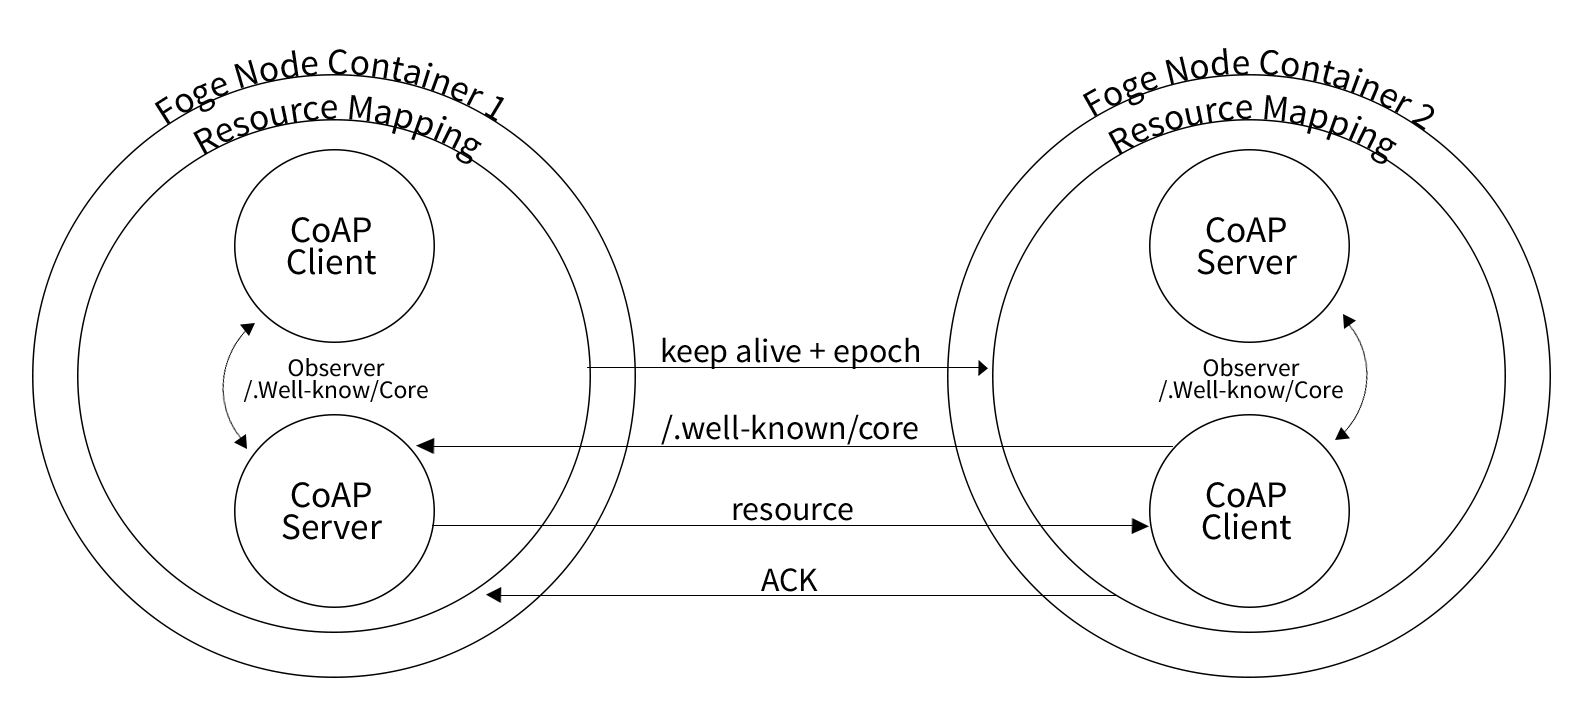
\includegraphics[width=.8\textwidth]{fig13.png}
    \caption%[This figure has a shorter caption now]%
    {\label{fig:fig13} Fog node container.}
\end{figure}


Além do protocolo de mapeamento em sí, este trabalho dispõe de uma API para o gerenciamento de recursos providos pelos CoAP servers.
Esta API possui métodos para listagem, remoção e criação de recursos e deve ser executada a partir do host que gerencia os container.
Assim, conseguimos proporcionar o dinamismo que a névoa necessita para a realização de testes no comportamento do protocolo de sincronização.



\section{Validações}
% Sergio: Essa seção, juntamente com os cenários de teste, podem fazer parte do capítulo 4

A validação deste trabalho consiste em realizar simulações que faça com que o protocolo execute suas funcionalidades de acordo com os resultados descritos na Seção anterior, sendo assim, 
algumas situações devem ocorrer para que as validações sejam realizadas.
Estas situações serão abordadas nos cenários de teste da Seção a seguir.

\section{Cenários de teste}

Utilizando como base a Figura \ref{fig:fig7}, e partindo do pressuposto que todos os nodos da névoa já estão com seus recursos sincronizados corretamente,
iremos exemplificar os cenários de testes elencados abaixo.

\begin{enumerate}
    \item Entrada de algum equipamento na rede e este anunciando seus recursos. 
    \item Atualização das listas globais quando algum equipamento deixar de responder as mensagens de keep alive.
    \item Atualização da lista de recursos quando algum edge device é adicionado ou removido de um nodo da névoa.
\end{enumerate}

\begin{figure}[H]
    \centering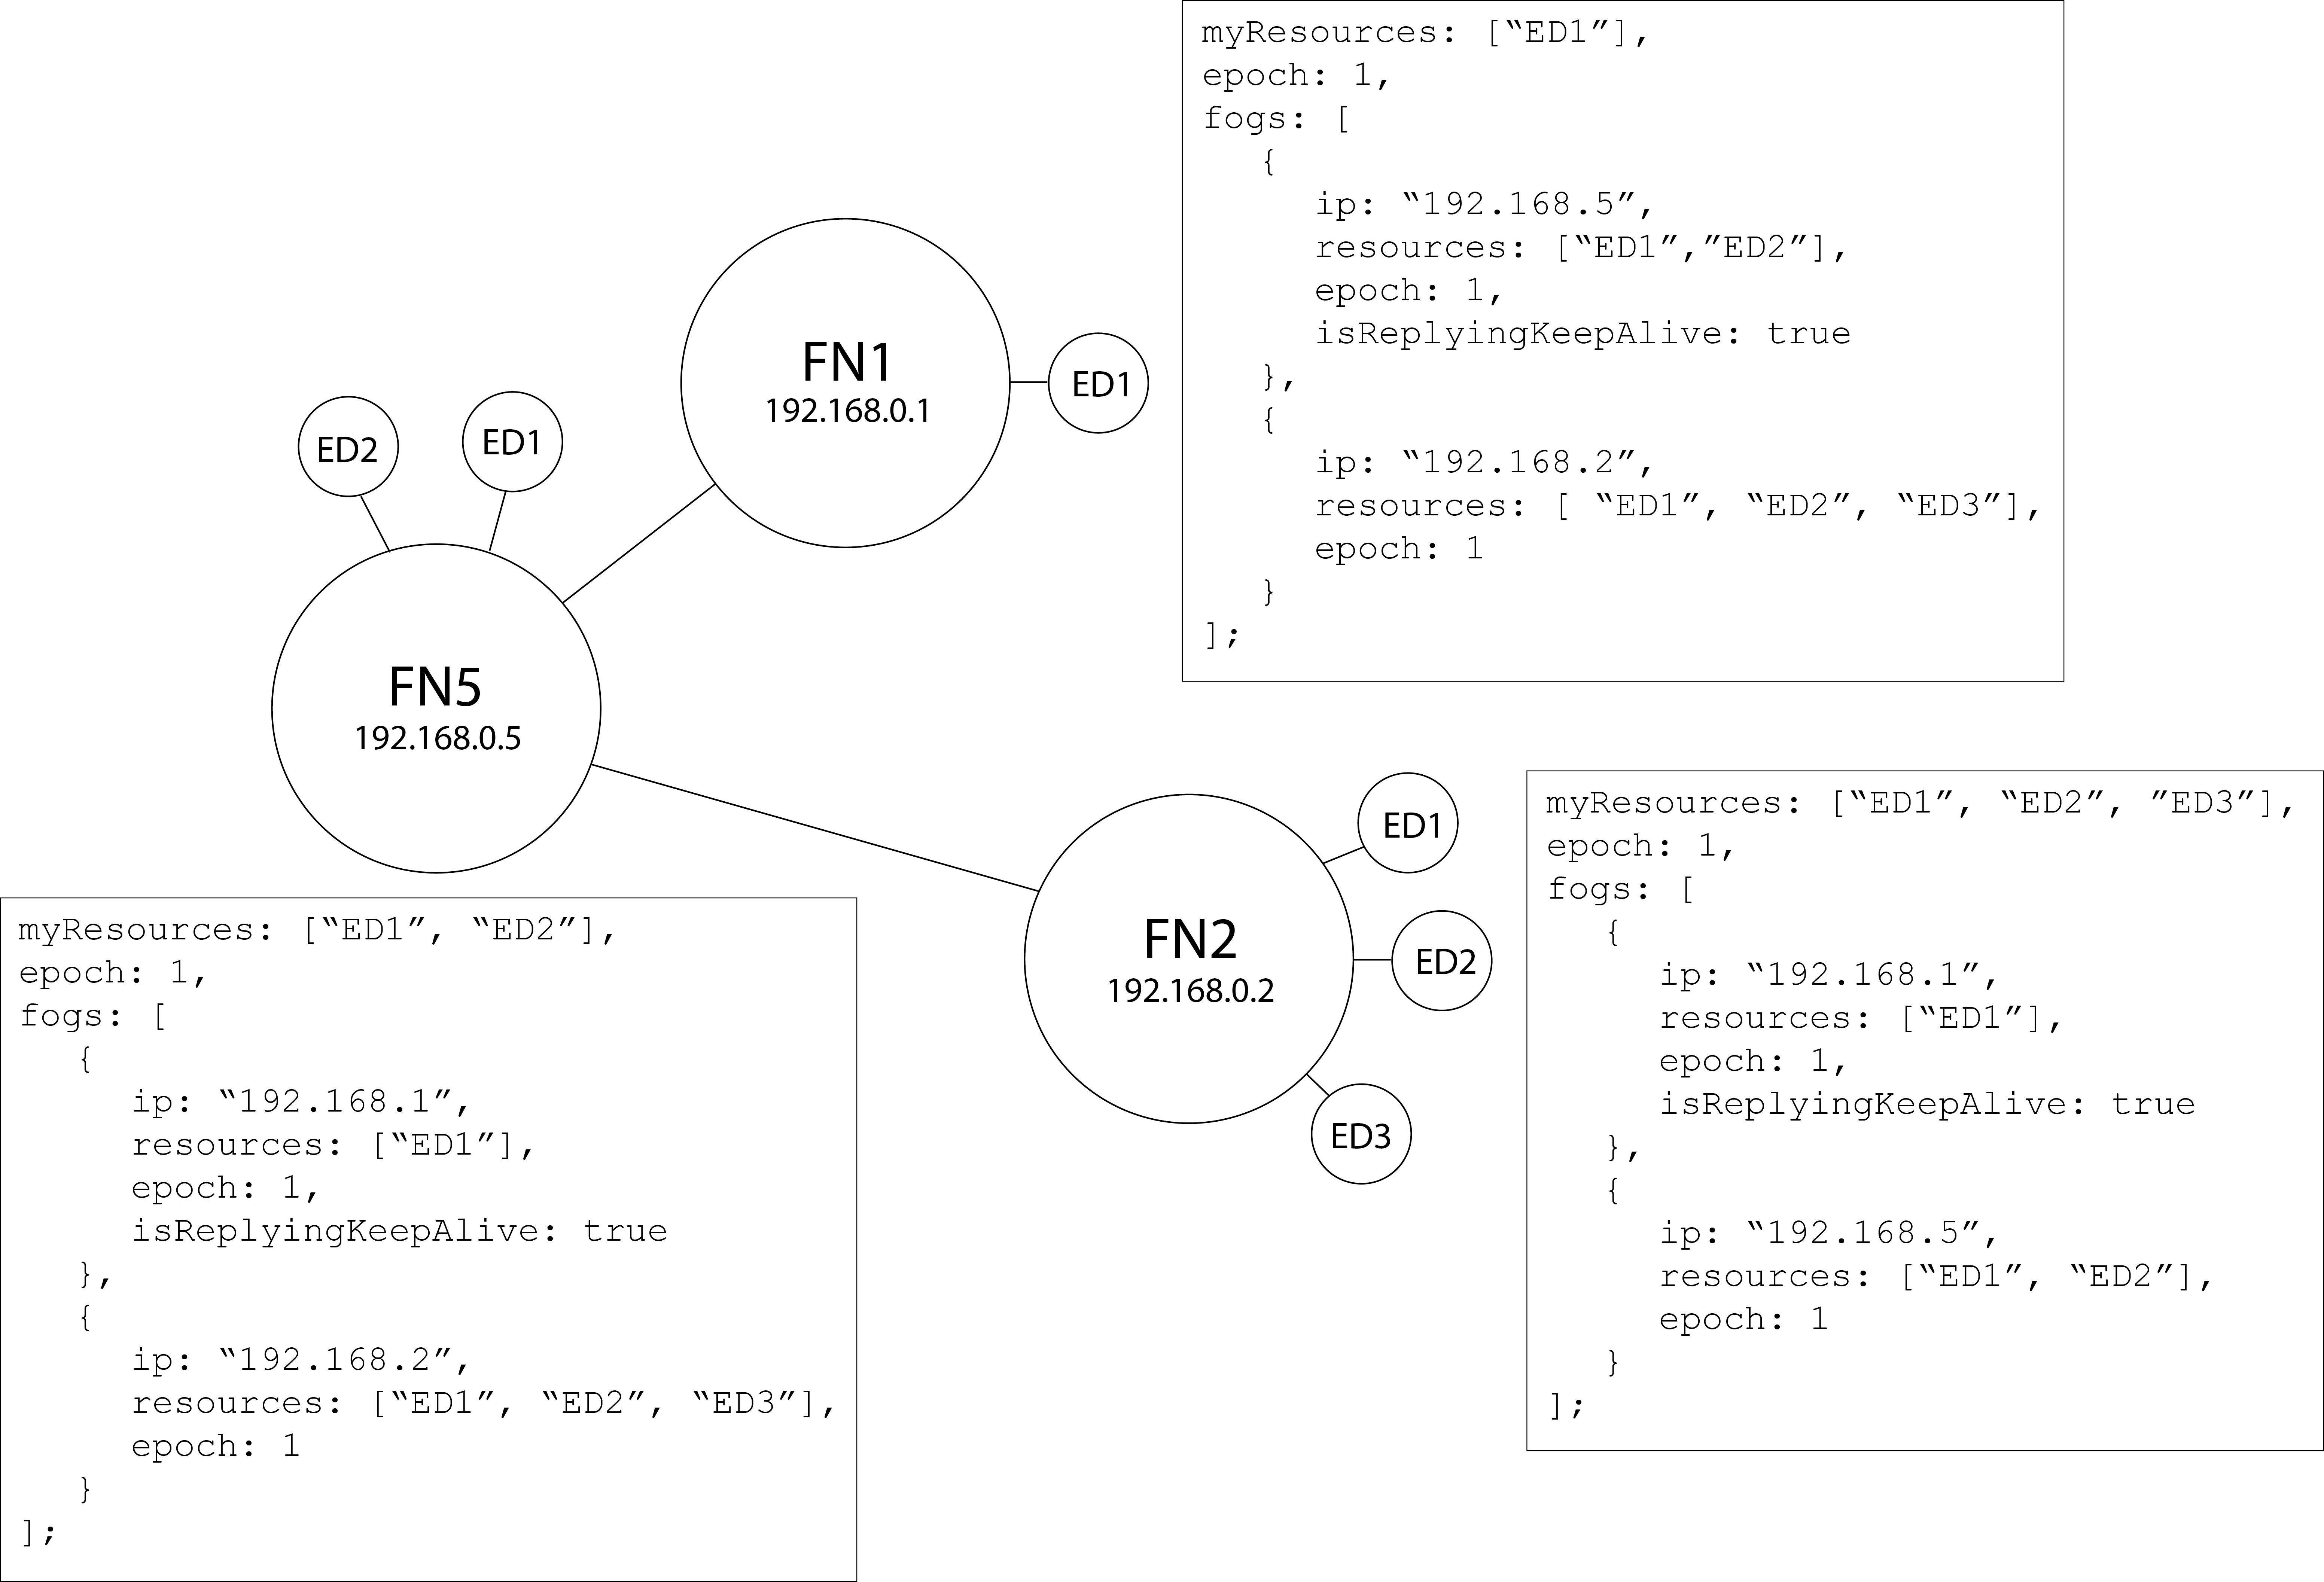
\includegraphics[width=.8\textwidth]{fig7.png}
    \caption%[This figure has a shorter caption now]%
    {\label{fig:fig7} Topologia base para cenário de teste.}
\end{figure}

O item 1 não será demonstrado agora, uma vez que as Subseções 3.2.2 e 3.2.3 já o fizeram, portanto, partiremos diretamente para o segundo item da listagem.

O segundo item trata-se de quando um nodo deixa de responder mensagens de keep alive, e a Figura \ref{fig:fig7} será utilizada para ilustrar este funcionamento.
Na Figura \ref{fig:fig8}, o nodo FN1 não respondeu, no tempo previamente estipulado, a mensagem de keep alive enviada pelo nodo FN2, 
portanto, o nodo destinatário foi marcado em FN2 como parcialmente inativo.


\begin{figure}[H]
    \centering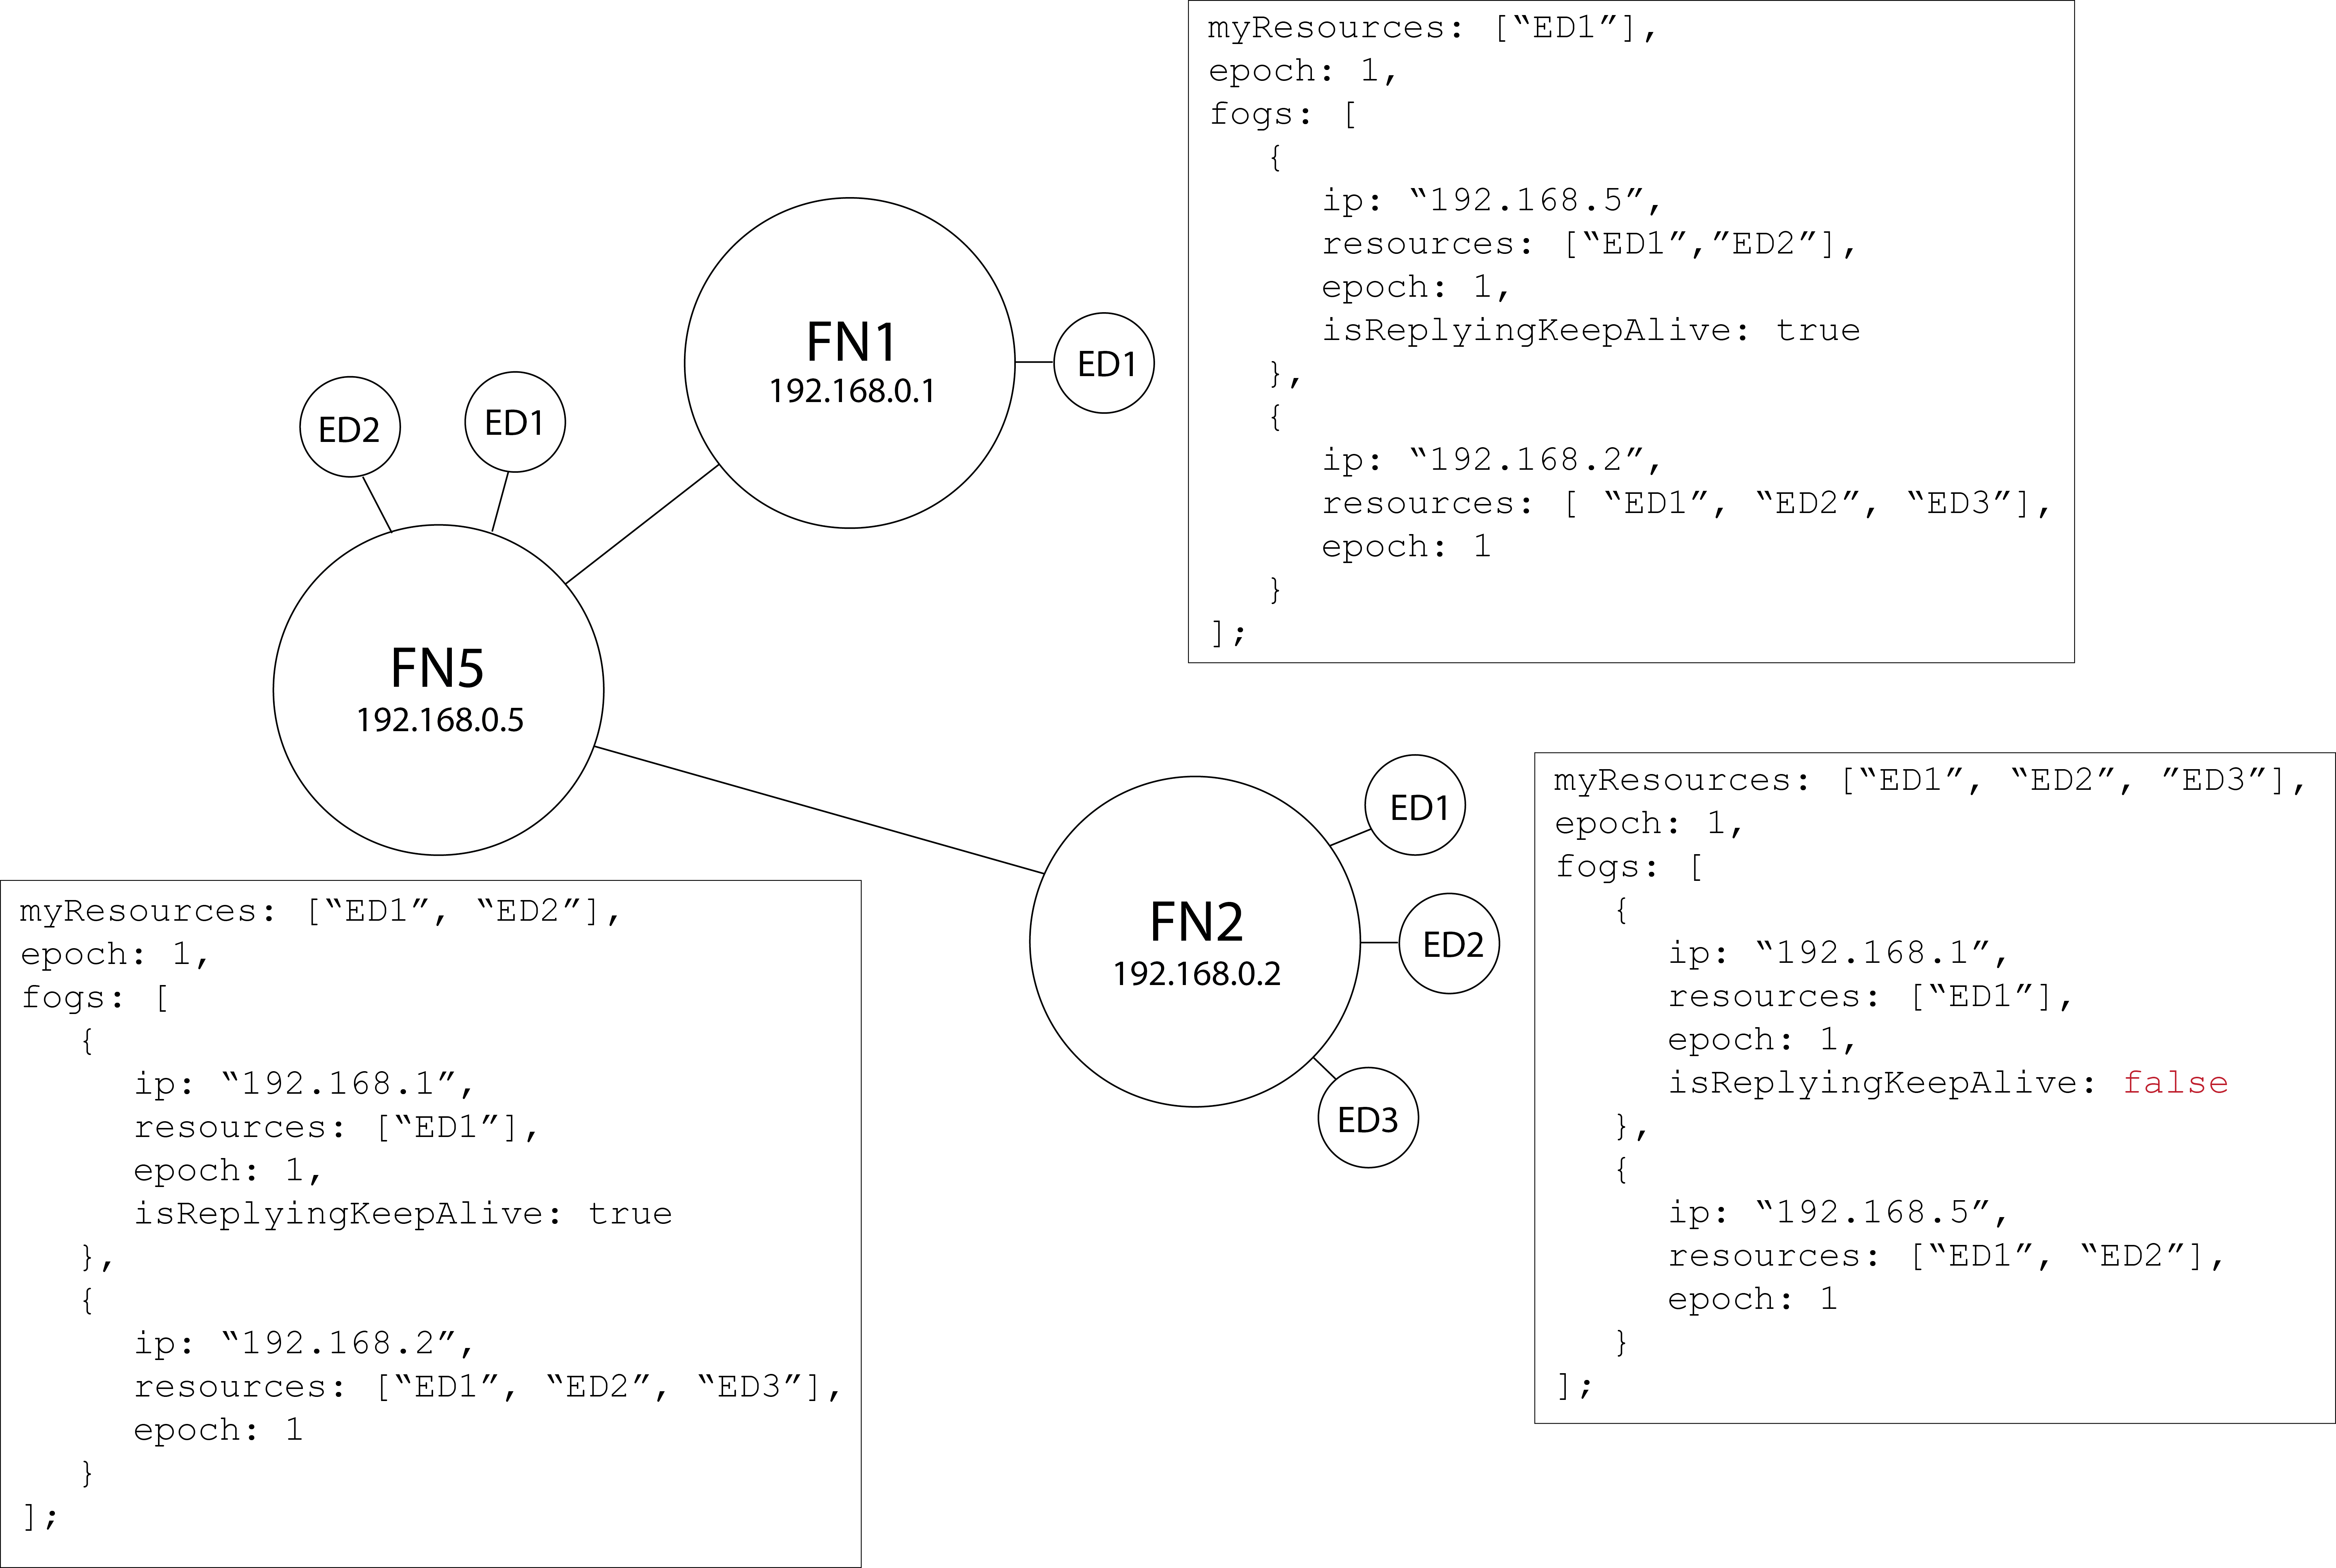
\includegraphics[width=.8\textwidth]{fig8.png}
    \caption%[This figure has a shorter caption now]%
    {\label{fig:fig8} Nodo marcado como parcialmente inativo.}
\end{figure}

Já a Figura \ref{fig:fig9} demonstra que o nodo FN1 não respondeu novamente à mensagem de keep alive enviada por FN2, por isso, foi removido de sua lista de recursos. 

\begin{figure}[h!]
    \centering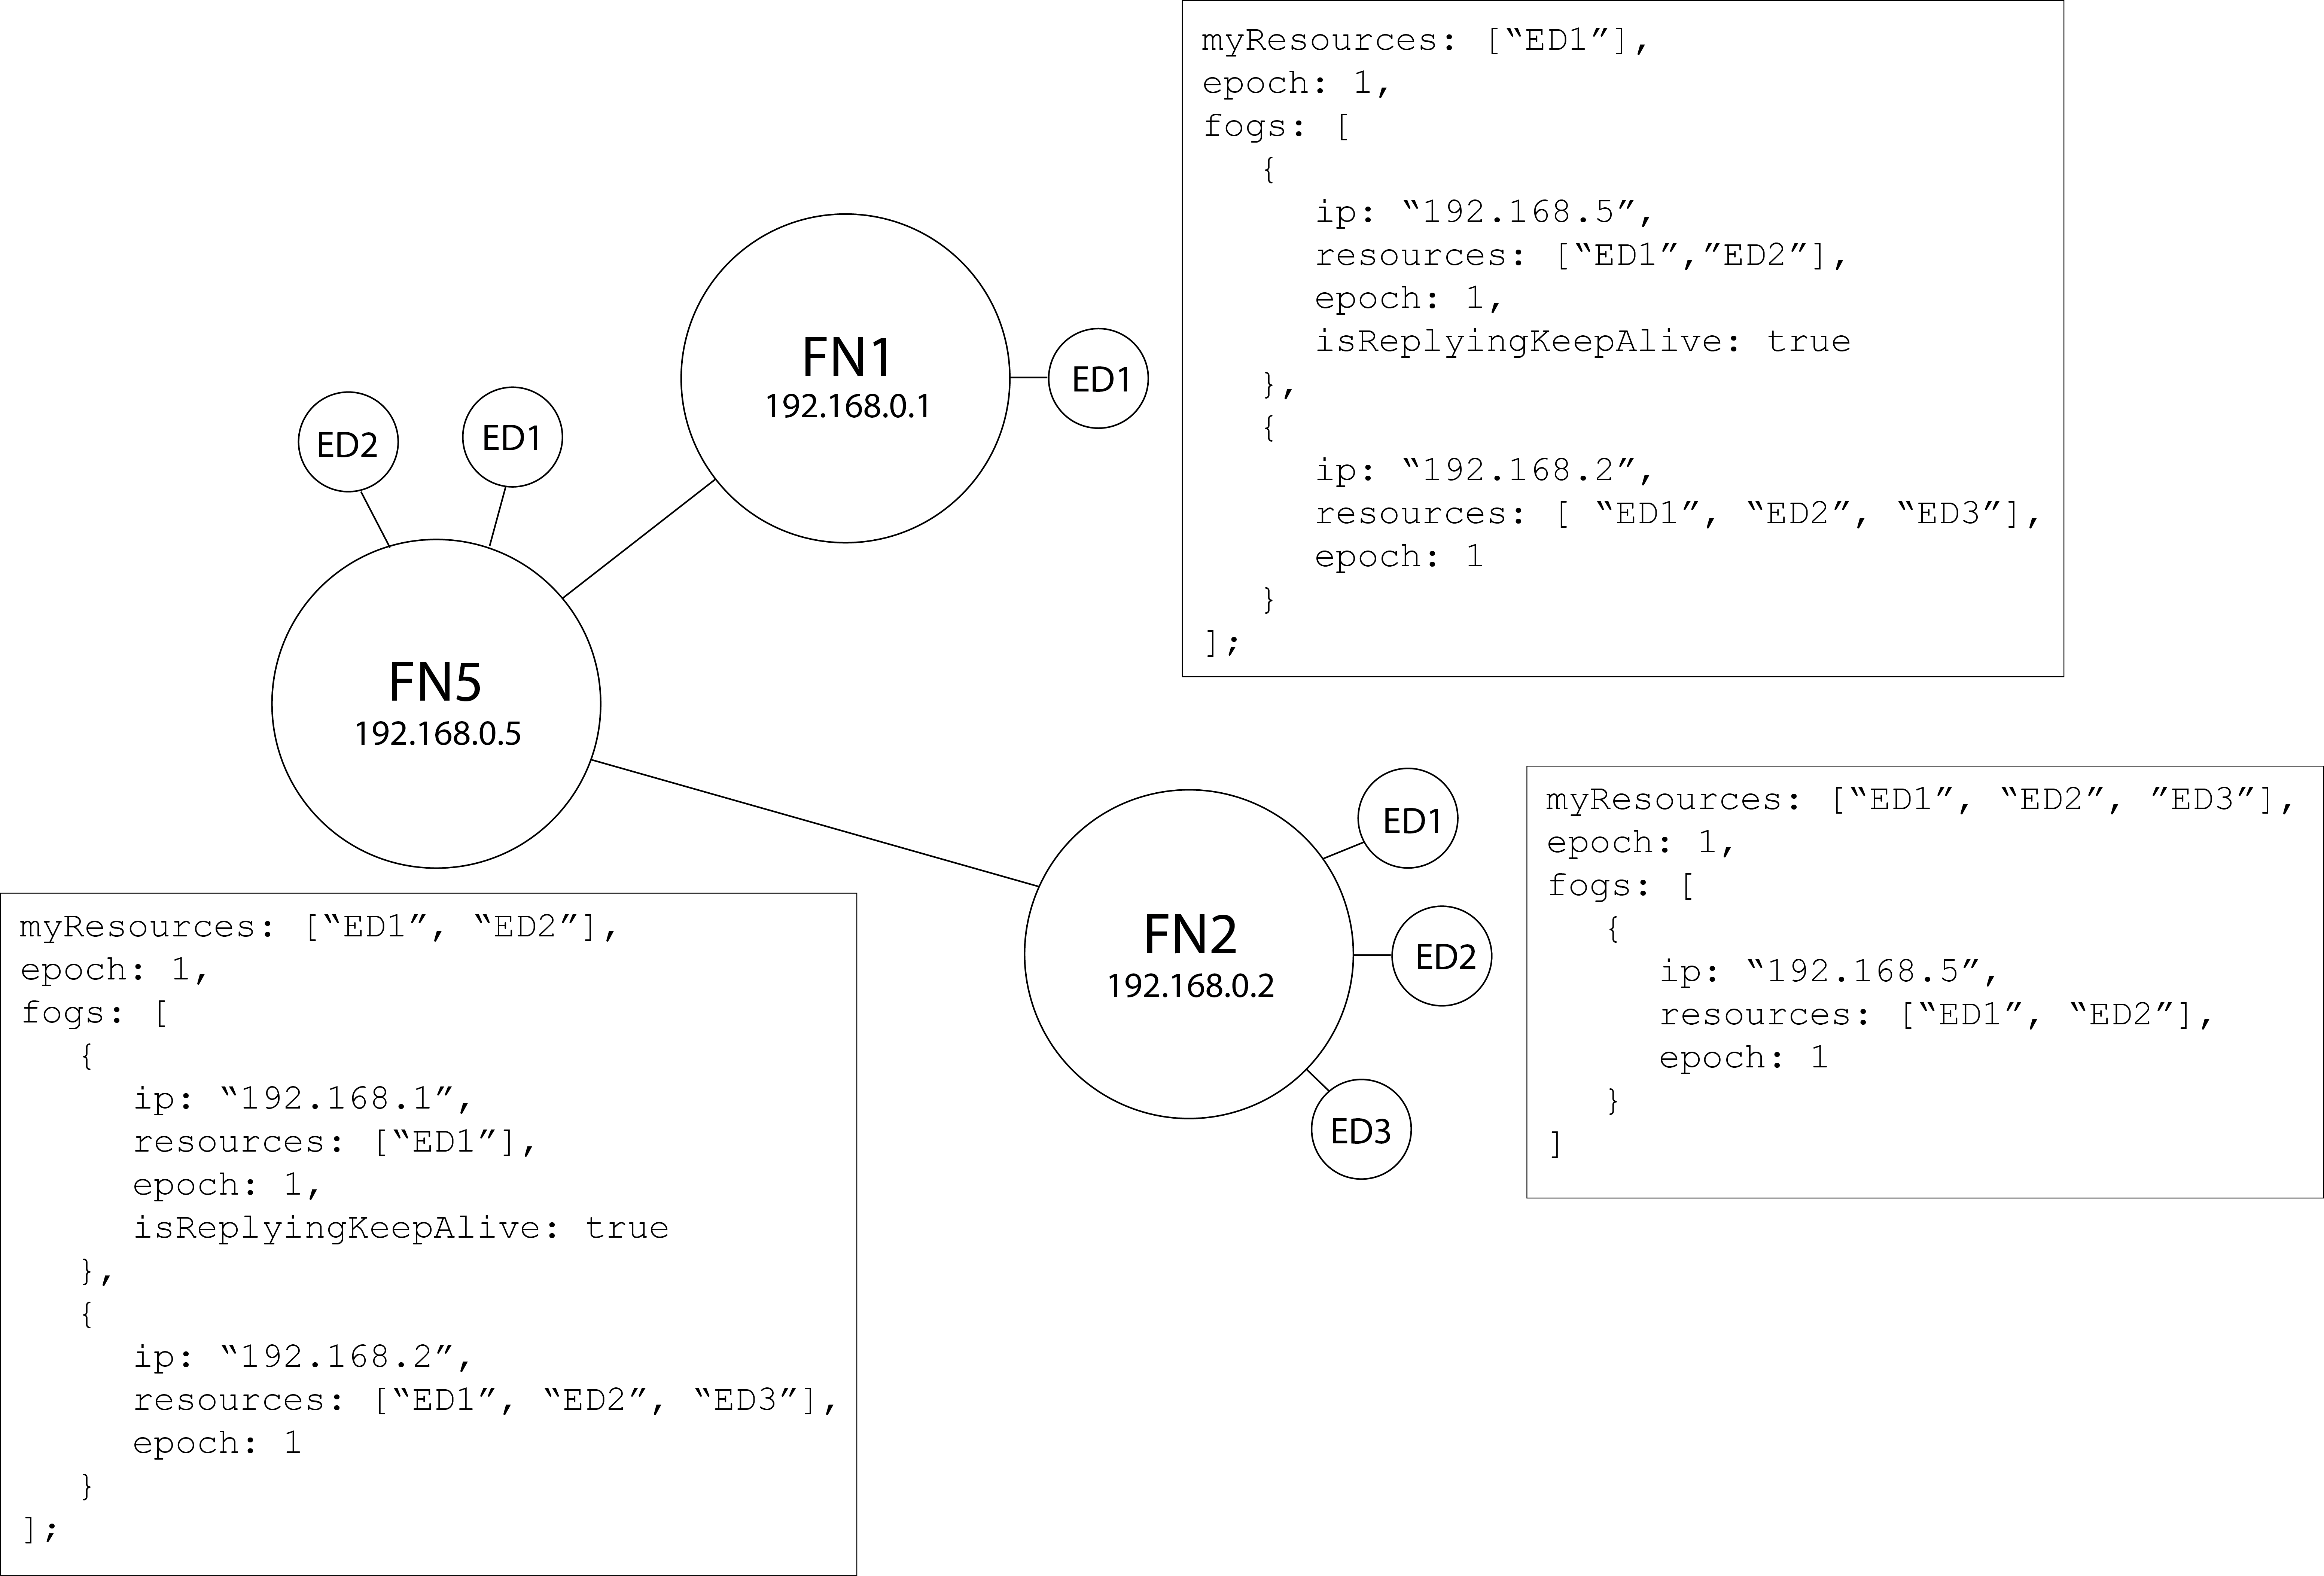
\includegraphics[width=.8\textwidth]{fig9.png}
    \caption%[This figure has a shorter caption now]%
    {\label{fig:fig9} Nodo removido da lista de recursos.}
\end{figure}

O terceiro item dos cenários de teste trata de quando o nodo está normalmente em operação, porém, um de seus recursos foi alterado, seja por incremendo de um novo edge device ou
pela remoção de um.

\begin{figure}[H]
    \centering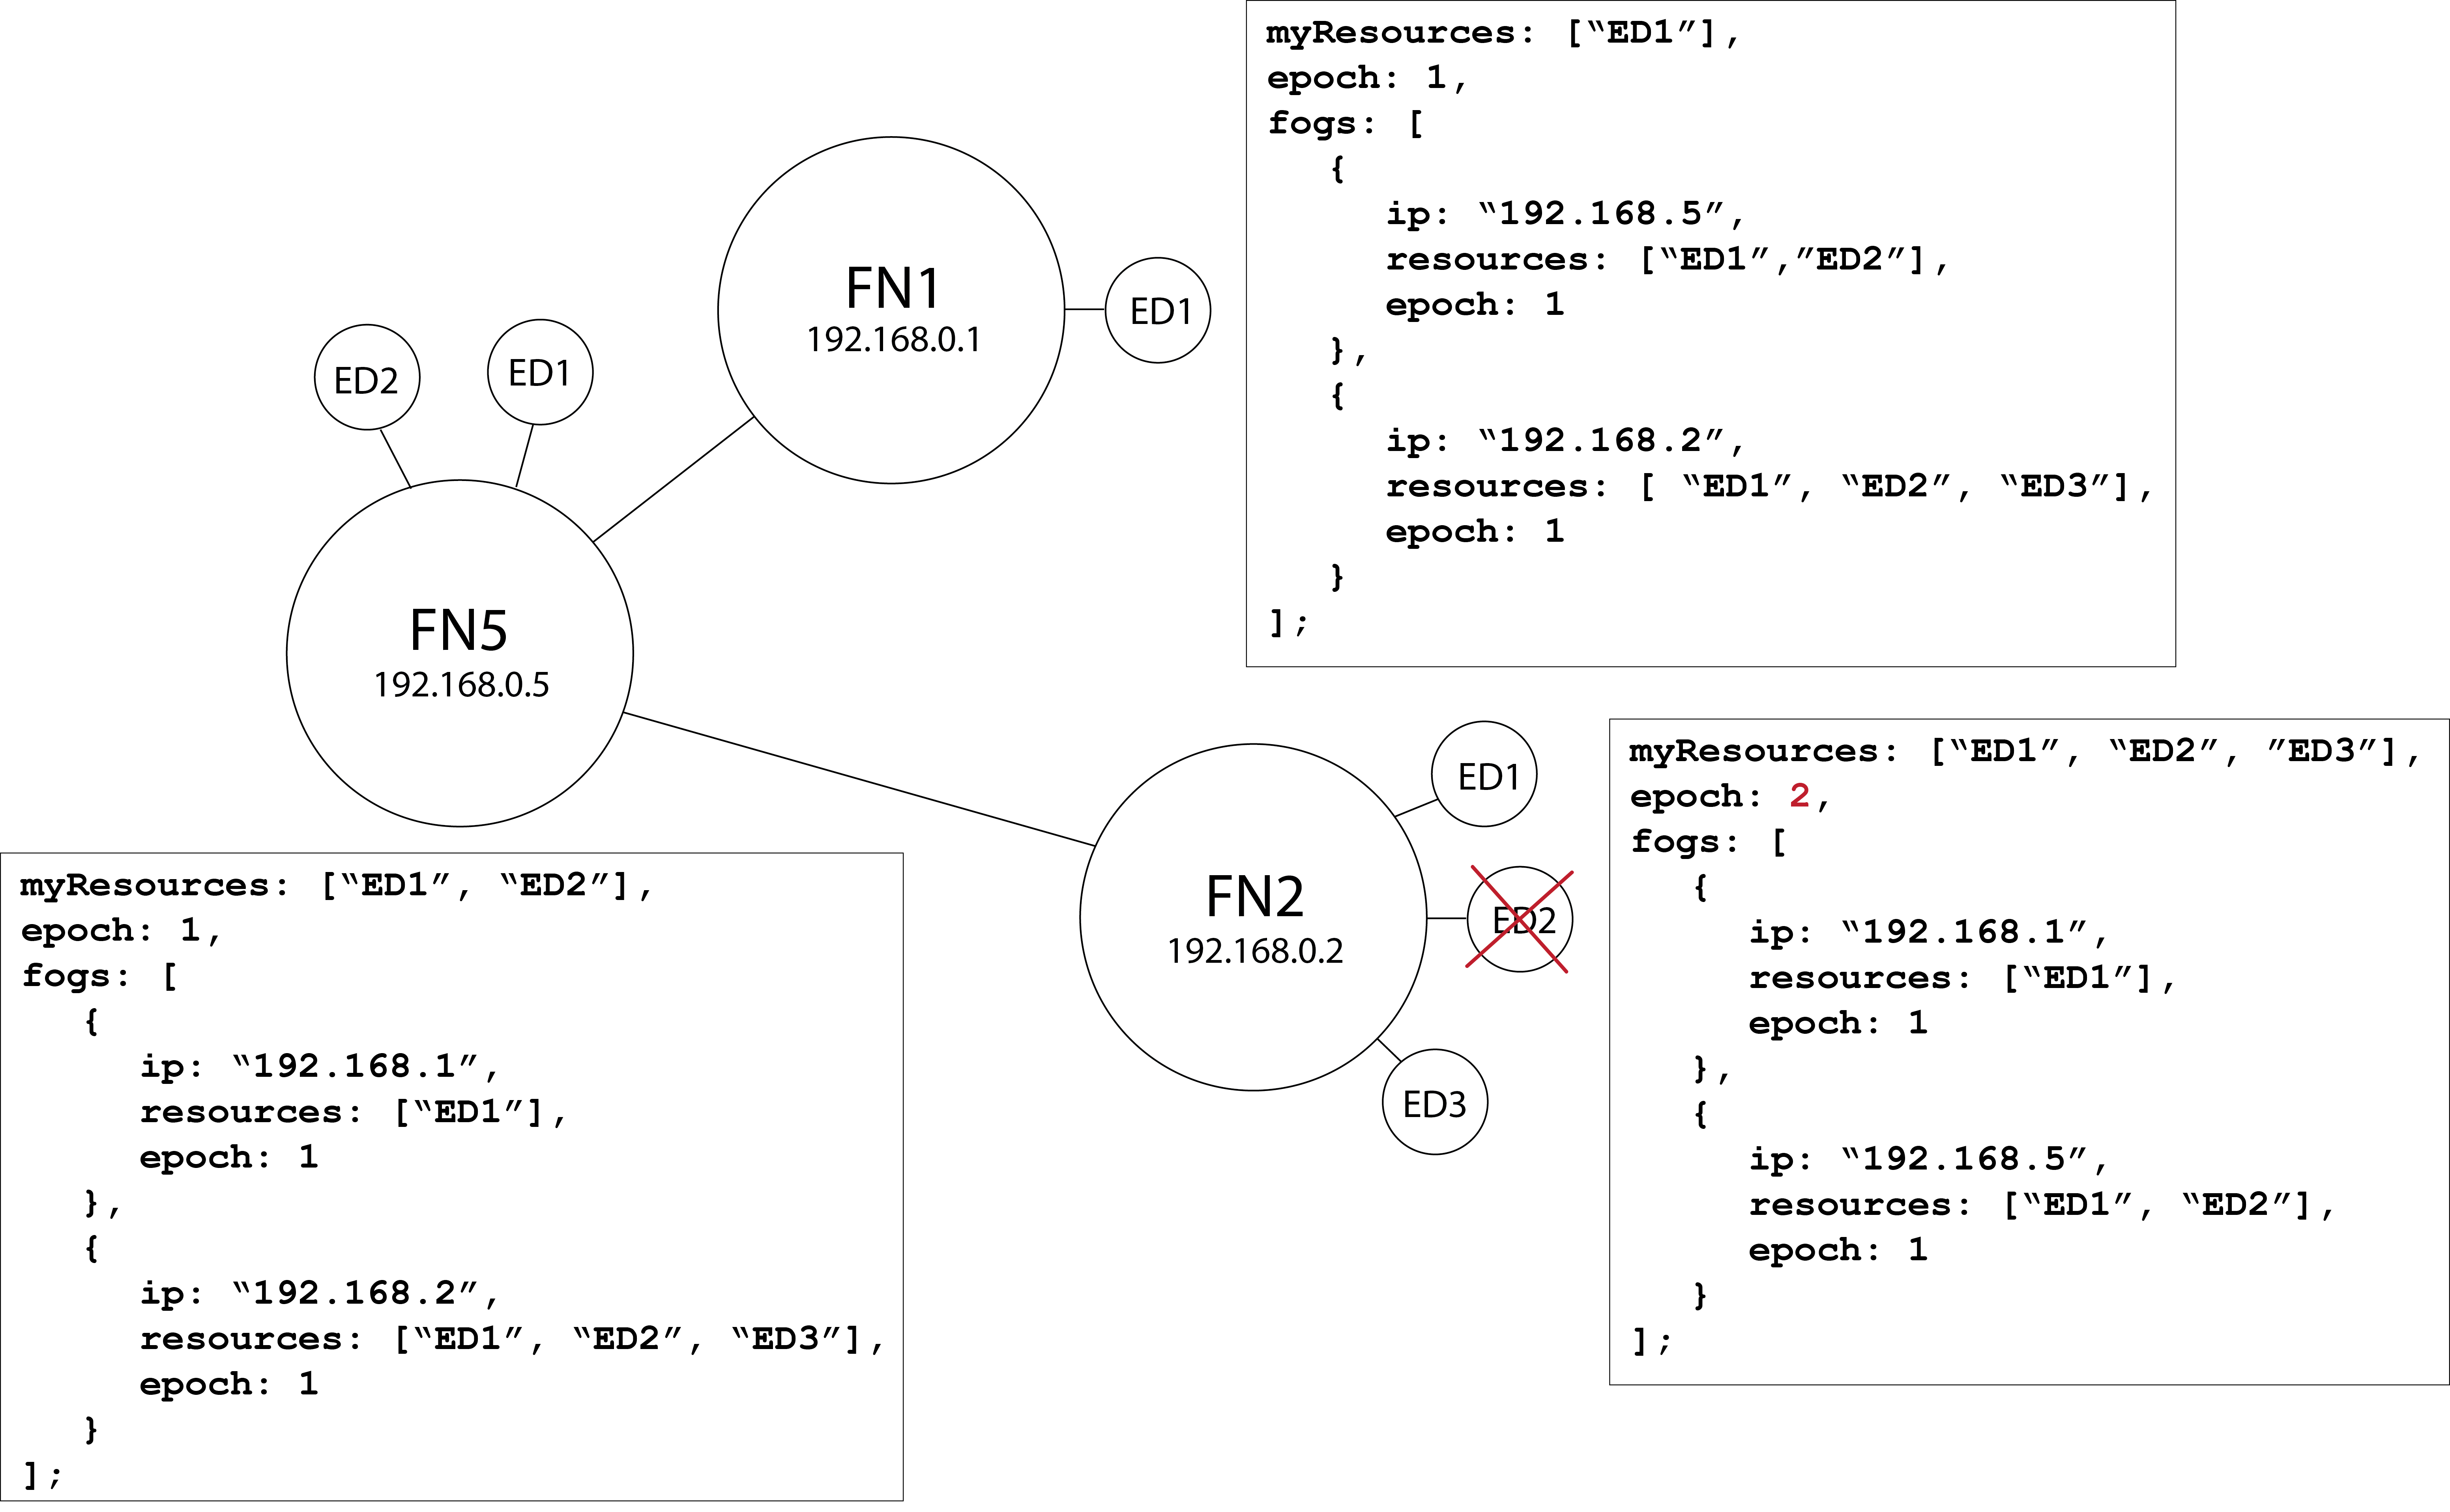
\includegraphics[width=.8\textwidth]{fig10.png} 
    \caption%[This figure has a shorter caption now]%
    {\label{fig:fig10} Edge device fora de operação.}
\end{figure}

Utilizaremos a Figura \ref{fig:fig10} como exemplo básico, e nela podemos observar que o edge device denominada ED2 vinculado ao nodo FN2 parou de funcionar.
Para este cenário, o nodo que hospeda ED2 deve estar ciente que este edge device está inoperante, e assim atualizar a sua \textit{época}.
O nodo que possui o edge device inoperante, então, terá sua época enviada juntamente com as mensagens de keep alive.
Assim, quando o nodo receber esta mensagem poderá comparar a época armazenada em sua lista de fogs com a época recebida pelo keep alive, e após a validação da divergencia realizará
um Requisição diretamente ao nodo para que possa atualizar sua lista de recursos globais.

\begin{figure}[H]
    \centering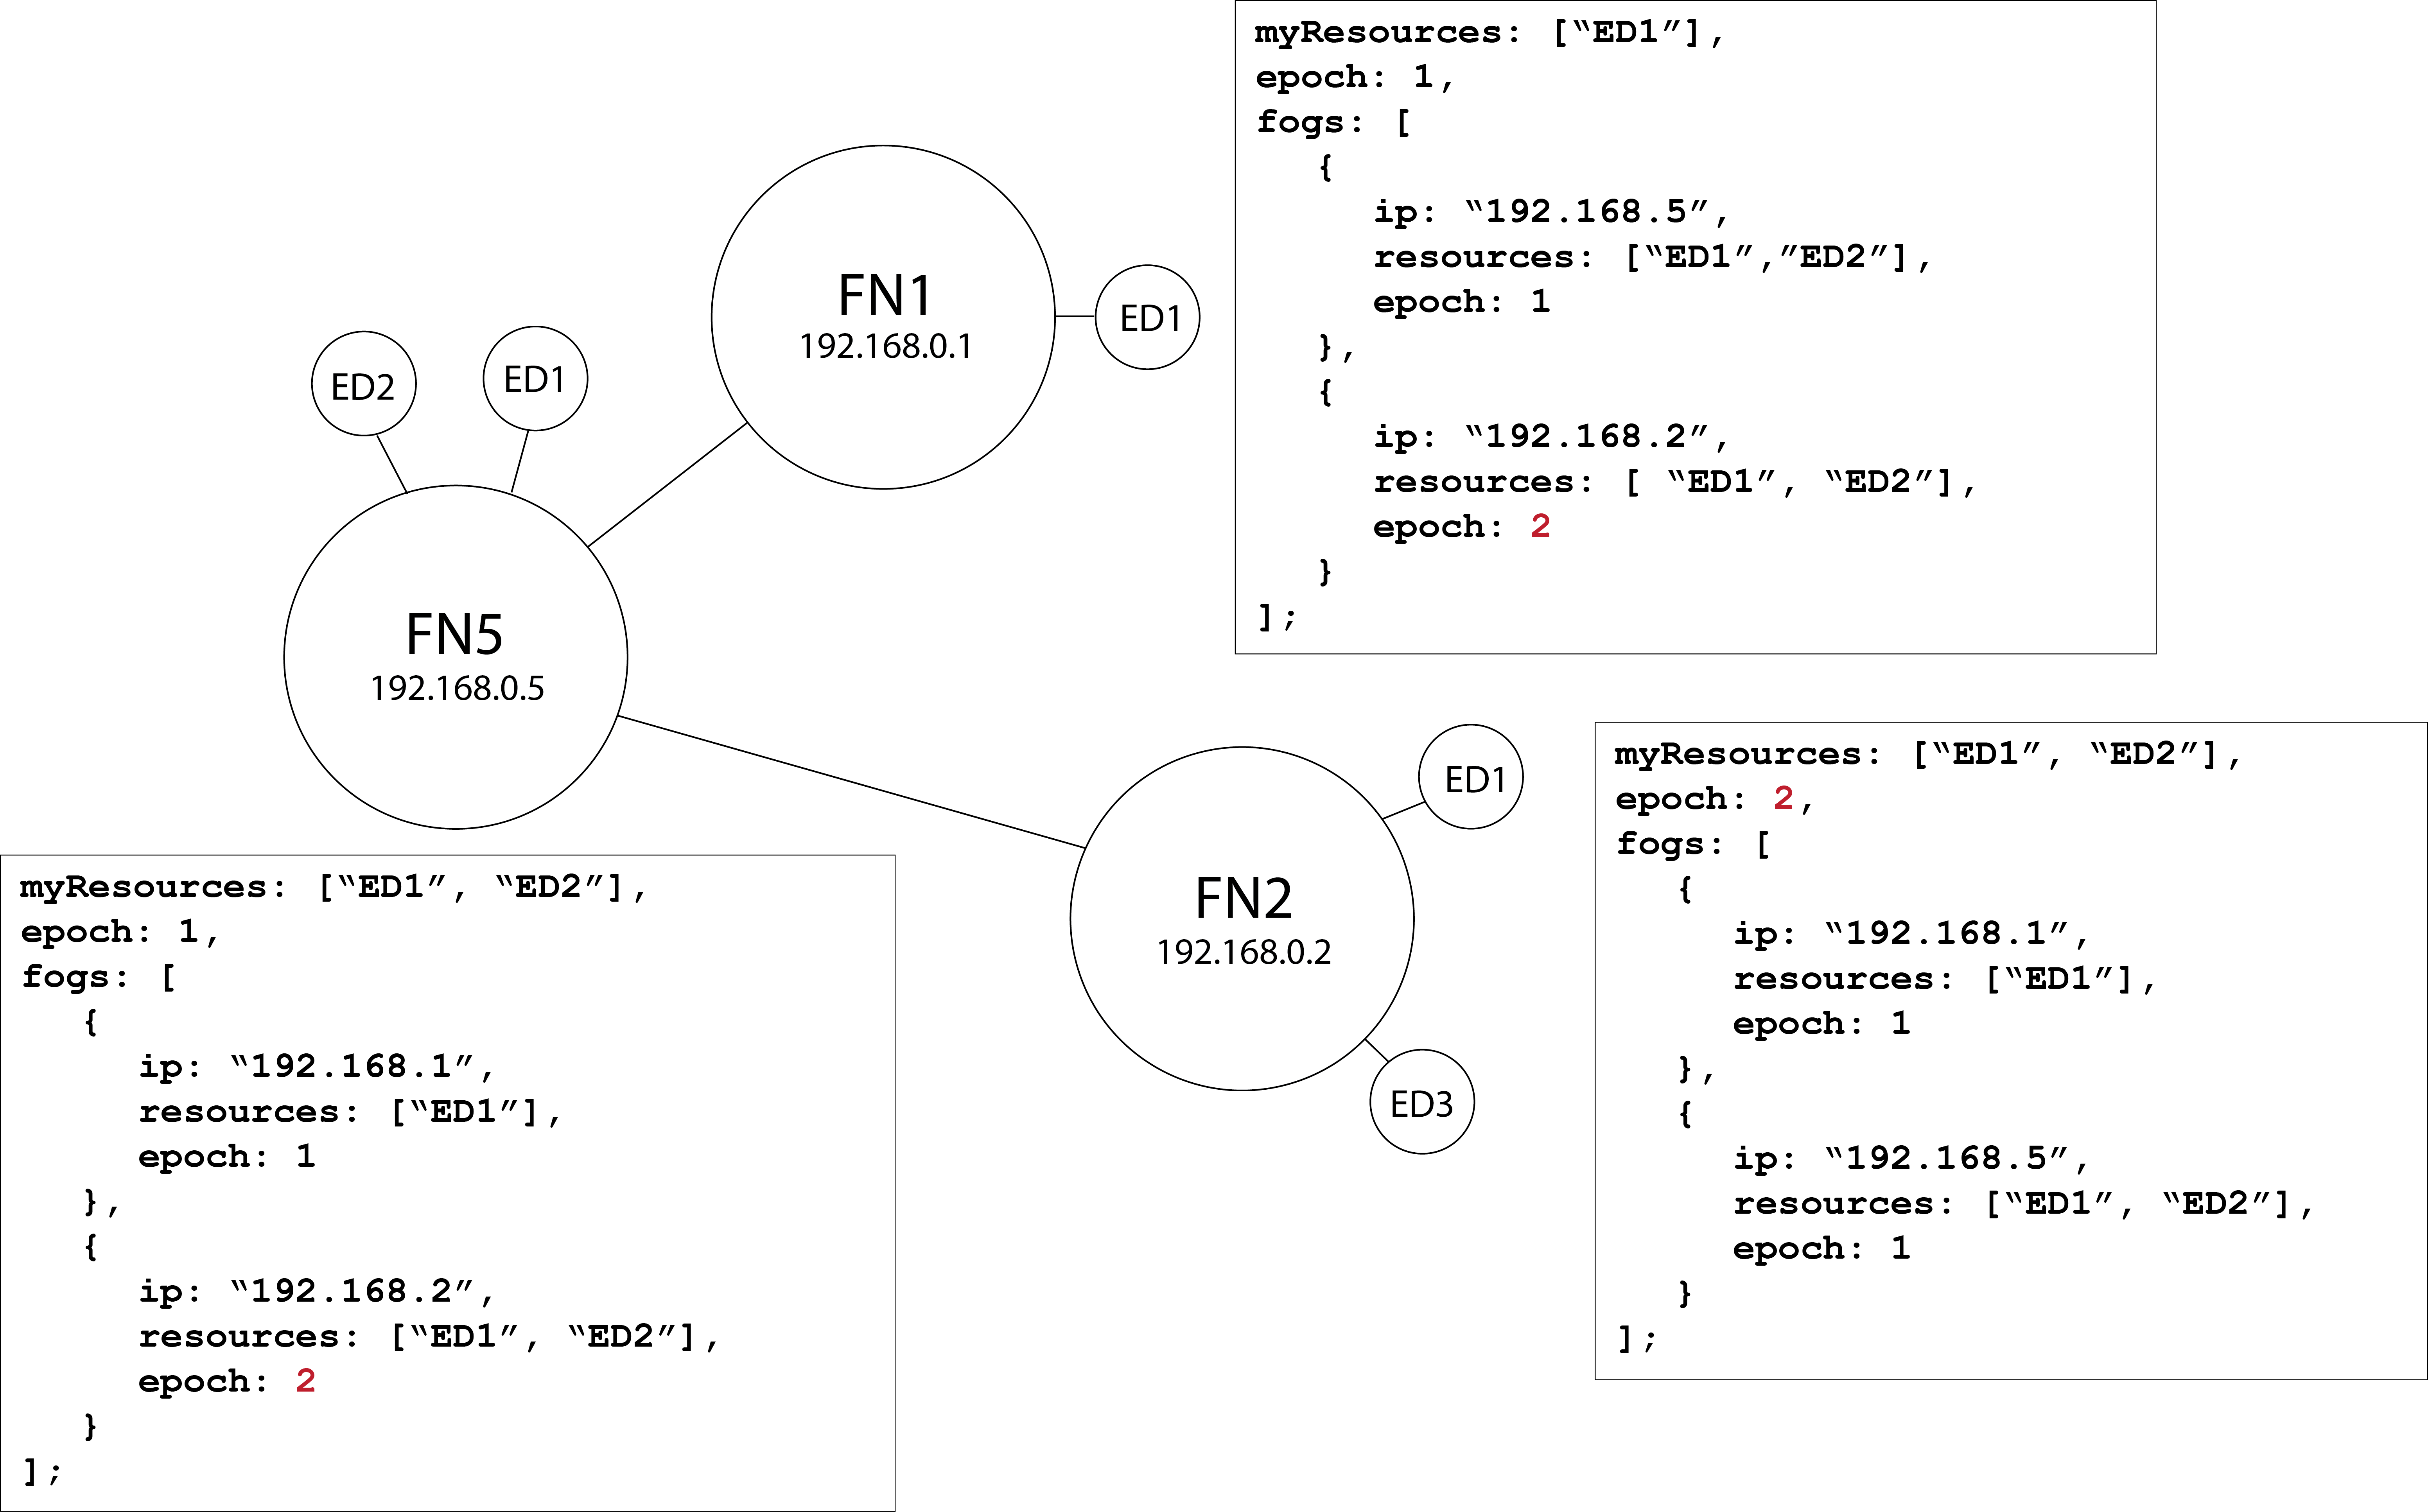
\includegraphics[width=.8\textwidth]{fig11.png} 
    \caption%[This figure has a shorter caption now]%
    {\label{fig:fig11} Estado da névoa após atualização de recursos.}
\end{figure}



